%Feb 5, 2014
%Draft outline: MSIP
%Chris Carilli
\documentclass[preprint]{aastex}

\usepackage[top=1in, bottom=1in, left=1in, right=1in]{geometry}
\usepackage{amsmath}
\usepackage{graphicx}
\usepackage{mdwlist}
\usepackage{natbib}
\usepackage{natbibspacing}
\usepackage{caption}
\usepackage{subcaption}
\setlength{\bibspacing}{0pt}
\setlength{\parskip}{0pt}
\setlength{\parsep}{0pt}
\setlength{\headsep}{0pt}
\setlength{\topskip}{0pt}
\setlength{\topmargin}{0pt}
\setlength{\topsep}{0pt}
\setlength{\partopsep}{0pt}
\setlength{\footnotesep}{8pt}
\pagestyle{empty}
\citestyle{aa}
\usepackage{enumitem}
%\usepackage[font=small]{caption}


\newcommand{\compress}{\vspace{-0.12in}}


\def\kperp{k_{\bot}}
\def\kpar{k_{\|}}
\def\nwnh{{\sl NWNH}}

\newcommand{\simgt}{\stackrel{>}{_{\sim}}}
\def\kperp{k_{\bot}}
\def\kpar{k_{\|}}
\def\k{{\bf k}}
\def\sky{{\theta}}
\def\HI{{H{\small I }}}
\def\HII{{H{\small II }}}
\def\xHI{{x_{\rm\HI}}}

%project description 20 pages total

\begin{document}

\title{Hydrogen Epoch of Reionization Array: Characterizing Cosmic Dawn}

\section{Overview} % 1 page ~ project summary? 
% Parsons, Carilli

% A statement of which of the four categories of MSIP is most appropriate
%for this proposal as the first sentence (see section II. Program Description).

%A. We propose HERA: next step in reionization roadmap
%B. Fulfill NWNH high-priority goals
%C. New understanding/techniques => faster, better, cheaper
%D. Brief summary of timeline: science along the way, major results before end-decade

{\it For the Mid-Scale Science Projects category of the Mid-Scale
Innovations Program}

The Hydrogen Epoch of Reionization Arrays (HERA) roadmap is a staged
program that uses the unique properties of the 21-cm line from neutral
hydrogen to probe the Epoch of Reionization and the preceding Dark
Ages.  During these epochs, roughly 0.3--1~Gyr after the Big Bang, the
first stars and black holes warm and reionize the neutral
intergalactic medium (IGM) that pervades the Universe following cosmic
recombination. Direct observation of the large scale structure of
reionization and its evolution with time, via the \HI 21-cm line, will
have a profound impact on our understanding of the birth of the first
galaxies and black holes, their influence on the intergalactic medium
(IGM), and cosmology.  CMB comparison statement? 

HERA was ranked the ``{\it top priority in the Radio, Millimeter, and
Sub-millimeter category of recommended new facilities for mid-scale
funding}" as part of the {\it New Worlds, New Horizons of Astronomy
and Astrophysics} decadal survey (\citealt{astro2010}; hereafter
NWNH).  The HERA roadmap initially envisioned a series of radio
interferometers constructed throughout the decade, starting with the
existing Donald C. Backer Precision Array to Probe the Epoch of
Reionization (PAPER) and the Murchison Widefield Array (MWA)
instruments aimed at characterizing foregrounds and laying the
groundwork for a statistical detection of the HI 21cm signal through
the power spectrum.  A second-generation HERA instrument would measure
the evolution of the power spectrum in detail and reveal how early
structure in the Universe formed. A third-generation instrument would
image the typical structures during reionization.

While receiving only a fraction of the funding for HERA phase I
recommended in NWNH, the MWA and PAPER projects have made
major strides in understanding the techniques required to disentangle
the reionization signal from the strong radio continuum foreground
confusion. Based on this new understanding of array response to the
celestial signal, we are ready to build the next generation of HERA in
stages of 127 and 331 elements, observing in the 50--225-MHz band.
These stages increase the sensitivity by two orders of
magnitude over the current arrays, through the use of an
optimal configuration of 14m diameter receptor elements, and a
tailored analysis technique that mitigates foreground contamination.
The proposed experiment delivers HERA-II science at a cost
substantially below originally envision in NWNH:

% XXX might remove 1st phrase in 1st sentence in para above

\vspace{-4pt}
\begin{itemize}\setlength{\parskip}{0pt}\itemsep0pt

\item HERA~127 will measure the rise and fall of the EoR power
spectrum, constraining the timing and duration of reionization.

\item HERA~331 will measure EoR fluctuations over a variety of spatial
scales to determine the features and distribution of the first objects
that dominate cosmic reionization. HERA~331 will also extend precision
power-spectrum observations into the Dark Ages, and directly image the
largest scale structures in the IGM during reionization.

\end{itemize}
\vspace{-4pt}

The proposed program produces a sequence of dedicated experiments
optimized to fulfill the NWNH goal of characterizing the evolution of
the HI 21cm power spectrum during cosmic reionization. In
its final stages, HERA may be capable of imaging the neutral
IGM --- a task previously only considered for third-generation
instruments. This proposal includes funding for both the
telescope development and construction, as well as for the key
scientific data analyses for each stage of the project.

\section{Science} total = 8 pages

\subsection{Introduction}    % 1 page + 1 fig = simulated Tb cube + PS evolution
% Furlanetto, Carilli

%i.physical concepts: reionization and dark ages
%ii. Current knowledge: various constrai	nts, 1st galaxy studies...
%iii. Important role of 21cm studies highlighted in NWNH
%a. Typical ideal sim results: T_B vs. z 'cube' and corresponding power spectrum evolution (Fig)
%b. introduce some of the important parameters/processes explored: when? how? bubble scale? sources? inside out? [much of this could be left for below?)
%c. reemphasize that current knowledge is nil, yet demand is high
%d. emphasize unique (only?) probe of dark ages

The {\it cosmic dawn}, or the period beginning with the the birth of the first stars and culminating with the full
ionization of the intergalactic medium (IGM) some 500 Myrs later, represents one of the last unexplored phases in 
the history of structure formation. During this period, a wealth of astrophysical and cosmological phenomena are at 
work. The characteristics of the IGM depend on (for example) the cosmic density field, the formation sites of the 
first luminous sources (e.g., their typical masses and clustering), their constituents (e.g., exotic Population III 
stars, more normal stars, stellar remnants, or supermassive black holes) their ultraviolet luminosities (which affect 
the IGM's ionization state), the efficiency and abundance of X-ray sources (which affect the IGM temperature), and 
even exotic effects like the relative velocity of baryons and dark matter.  Exploring these early structures and their 
effects on each other and their environments was one of the top three ``{\it priority science objectives chosen by 
the [NWNH] survey committee for the decade 2012-2021.}"

%SF: This next paragraph worries me a bit because most of these probes have one or several competing groups working 
%on them, and if we get a referee from one of the groups we don't reference they might get pissy...right now 
%I've tried to be fair but terse here
Observations are now just beginning to penetrate into this early epoch, primarily at its tail end.  Recent 
measurements from the {\it Hubble Space Telescope} have pinned down the bright end of the galaxy luminosity function 
at $z \la 8$ \citep{bouwens_et_al2010, schenker_et_al2013} and begun to detect a few sources at even greater 
distances \citep{ellis_et_al2013, oesch_et_al2013}.  Meanwhile, a number of indirect probes have placed constraints -- 
albeit model-dependent ones -- on cosmic reionization, as summarized in the left-hand panel of 
Figure~\ref{fig:x_i_Xray}. These include observations of resonant scattering of Ly$\alpha$ by the neutral IGM toward
distant quasars (the 'Gunn-Peterson' effect) \citep{fan_et_al2006}, the demographics of Ly$\alpha$ emitting 
galaxies \citep{schenker_et_al2012, treu_et_al2013, Capak_et_al2014}, and Ly$\alpha$ absorption near the most distant quasar 
\citep{bolton_et_al2011}, as well as measurements of CMB temperature fluctuations \citep{planck_et_al2013}, 
polarization anisotropies \citep{page_et_al2007}, and secondary temperature fluctuations generated by the 
kinetic Sunyaev-Zel'dovich effect \citep{zahn_et_al2012_trunc, mesinger_et_al2012}.  Reionization models can be 
built from galaxy observations.  Recent examples suggest that the IGM may have been substantially neutral even at 
$z \sim 7$--8 (as high as $F_{HI} \sim 0.5$), with a tail of finite ionization ($\sim 0.1$) extending to high 
redshift ($z \sim 15$), driven by very early galaxy formation \citep{robertson_2013}.  The extrapolation to 
$z>8$ is particularly uncertain, as only a handful of candidate galaxies have been found during that earlier 
era (c.f. \citealt{oesch_et_al2013}).  Unfortunately, these important methods have limited reach: strong assumptions 
are required about the stellar populations and escape fraction of UV photons from the galaxies, while astrophysical 
constraints on reionization are highly model-dependent and the CMB provides only an integral measure of the process. 
Moreover, many of these indirect observations are in tension with one another, underscoring both the difficulty in 
their interpretation and the complexity of the reionization process.

The 21-cm ``spin-flip" transition of  neutral hydrogen has been recognized as potentially the most powerful probe 
of cosmic reionization and  the dark ages \citep{morales_wyithe2010, furlanetto_et_al2006}, as emphasized in NWNH: 
``{\it 
%SF: Is this quote from the RMS panel?  If so, does it appear in the final report?
The panel concluded that  to explore the discovery area of the epoch of reionization, it is most important to 
develop new capabilities to observe redshifted 21-cm \HI emission, building on the legacy of current projects and 
increasing sensitivity and spatial resolution to characterize the topology of the gas at reionization.}"  Because 
the Universe is almost entirely neutral before reionization, the HI 21-cm line provides a direct method to image 
the evolution of the primordial IGM, opening a unique window into the complex astrophysical interplay between the 
first luminous structures and their surroundings. Moreover, because of the cosmological redshift, we can associate 
the signal at each observed frequency with a particular emission time (or distance) and reconstruct a complete 
three-dimensional picture of the time evolution of large scale structure during this 'last frontier' in 
observational cosmology. 
%SF: Personally I feel like the following is an exaggeration that could rub some people the wrong way!
The direct observation of the primordial IGM via the HI 21-cm line would be an achievement comparable in importance 
to the detection of anisotropies in the CMB.

In the past decades, considerable effort has gone into modeling the complex astrophysics of reionization
(e.g. \citealt{shapiro_giroux1987, haiman_loeb1997, furlanetto_et_al2004, santos_et_al2010}). Figure ?? shows a 
simulation of the expected evolution of the HI 21cm signal during reionization. The HI 21-cm fluctuations initially 
rise above those expected from the cosmic density field due to the growth of ionized bubbles on a characteristic 
scale of a few to 10~arcmin. This scale is set by the clustering of early galaxy formation, as well as by 
propagation effects through the IGM. The signal then declines as the IGM becomes fully ionized.  These theoretical 
models of the reionization process are sophisticated and appear to be well-understood, {\it but they are not 
predictive tools.} Instead, they provide a mapping between the largely unknown galaxy populations and observables 
like the 21-cm transition. As such, the key questions about the cosmic dawn era remain poorly understood.  When 
did reionization occur, and over what timescale?  What objects dominated the radiation field?  How were the 
objects distributed?  What were the most important feedback mechanisms in the transition from the first stars to
first galaxies, and how did they affect these populations?  {\it HERA provides the key measurements that are needed 
to advance our understanding of early galaxy formation and cosmic reionization.}


Figures: F(HI) vs z;  HI Tb cube + PS evolution


\subsection{HI reionization and dark ages science} % 4 pages total examples using hera 331, plus a number of figures

i. F(HI) vs. z: HERA vs. other techniques (Fig) -- emphasize constaints in unexplored territory
% Bowman


\subsubsection{Detecting and characterizing the power spectrum}
\emph{ii. PS sensitivity at fixed z: 127, 331 (Fig)}
% Pober, Dillon
\begin{figure}[t]\centering
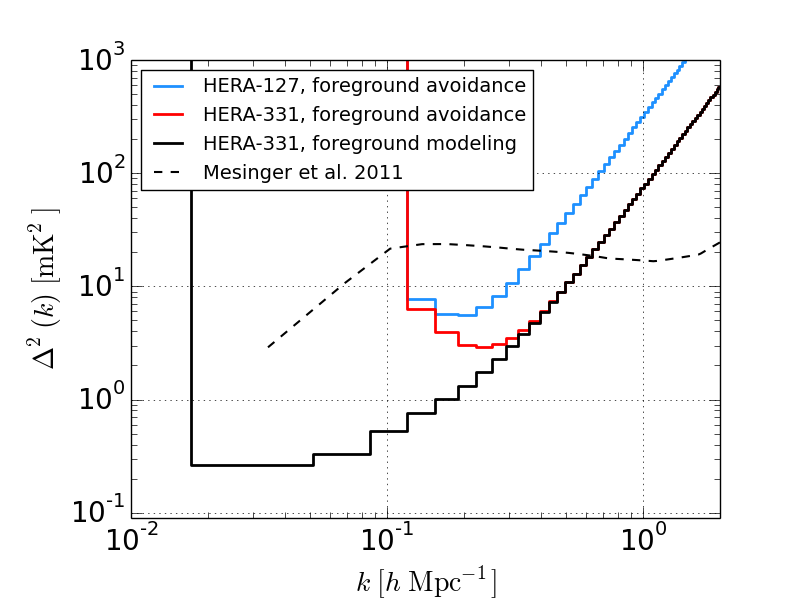
\includegraphics[width=\textwidth]{plots/Pspec/eor_pspec_2014.png}
\caption{Power-spectrum sensitivities for three stages of
HERA (solid) relative to a fiducial ionization model (dotted line; $\xHI=0.37$, $z=9.0$).  
Sensitivity curves reflect a staged array size and
a staged improvement in analysis software that expands the range
of modes falling into the EoR Window \label{fig:PspecSensitivity}}
\end{figure}

A season of observing with HERA-127 will yield high-significance constraints on the 21 cm power spectrum across a wide range of k modes and redshifts.  In Figure we show the $z=9$ power spectrum predicted by the publicly available 21cmFAST software \citep{mesinger_et_al2011}, along with $2\sigma$ HERA sensitivities.  Using the conservative delay-spectrum approach employed in Parsons et al. 2014, we find that HERA-127 can achieve a $> 10\sigma$ detection of fiducial power spectra over a broad range of redshifts.  The subsequent observing season with HERA-331 can increase this detection significance to over $25\sigma$ using the same methods.  With detailed foreground modeling, a more sophisticated power spectrum estimator could increase the size of the ``EoR window", the region of Fourier space with minimal foreground contamination. This would allow for an overall detection significance of up to $90\sigma$, along with access to lower $k$ modes and therefore qualitatively different physics.  Such a high 
sensitivity measurement would also allow one to go beyond constraining parameters, testing rather than assuming the underlying theoretical framework.

\subsubsection{Astrophysical parameters from the power spectrum}
\emph{iii. Various covariance analyses: constraints on different physical processes (Liu/Pober analysis). but
please -- keep this down to a couple of incisive figures and fiducial models. wall paper doesn't sell very well. }
% Liu, Pober, Dillon
The power spectrum measurements with HERA-331 are sensitive enough to place constraints on theoretical models that describe the reionization process.  To first order, the major features of the power spectrum (as simulated by 21cmFAST) can be parameterized by three terms: $\zeta$, the efficiency at which galaxies release ionizing photons into the IGM; $T_{\rm vir}$, the minimum virial temperature of halos that produce ionizing photons (a proxy for the minimum mass of the galaxies that drive reionization); and $R_{\rm mfp}$, the mean free path for ionizing photons traveling through the IGM, which is determined the prevalence of dense Lyman limit systems.  Current observations limit the value of these parameters to within an order-of-magnitude (or worse, in the case of $T_{\rm vir}$).  Figure \ref{fig:ErrorEllipses} shows the constraints on each of these parameters achievable with multi-redshift HERA-331 power spectrum observations.  We expect to constrain these parameters to better than 5\% with a conservative 
approach to foregrounds , and even better with explicit foreground modeling \citep{pober_et_al2014}.

\begin{figure*}[t]\centering
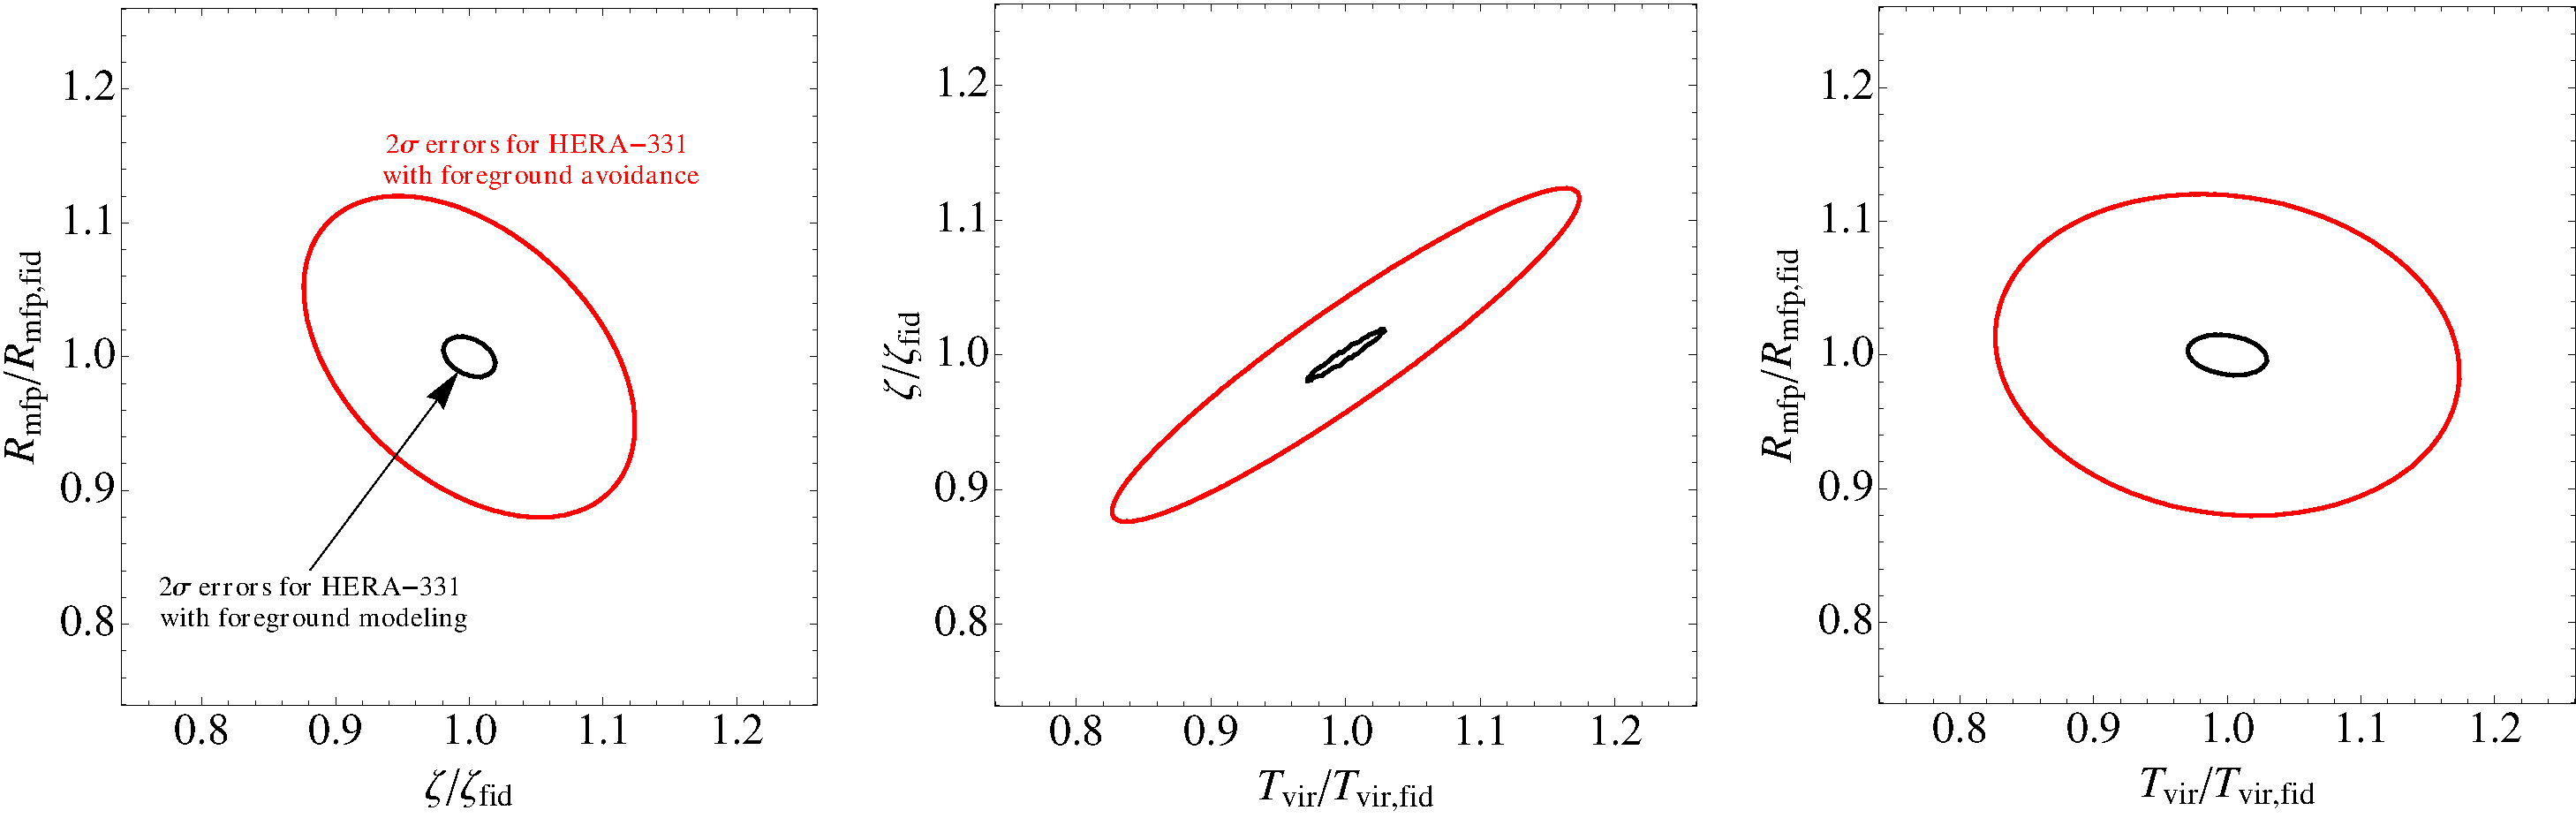
\includegraphics[width=\textwidth]{plots/Pspec/OPTMIDellipses.pdf}
\caption{Pairwise $2\sigma$ error ellipses for $T_{\rm vir}$, $\zeta$, and $R_\textrm{mfp}$, in each case divided by their fiducial values.  HERA-331 projections using existing foreground avoidance techniques are shown in red, while projections using more advanced foreground modeling techniques are shown in black.  The former represent $\sim 5\%$ constraints, while the latter represent $\sim 1\%$ constraints.\label{fig:ErrorEllipses}}
\end{figure*}


% Jacobs
\subsubsection{Imaging HI}
iv. Imaging large scale structure: simulation (Fig) 
With a nearly completely sampled aperture over 300m across, HERA will have the collecting area of Arecibo but with 500x the survey speed it presents the opportunity for directly imaging reionization.  After 100 hours on a single field (achievable in 200 nights, or just over one season) HERA will reach a surface brightness sensitivity of 50 $\mu$Jy compared with typical brightness temperatures of EoR models which often peak above 400 $\mu$Jy.

In imaging, as in the measurement of the power spectrum, noise and foreground residual are comparable limiting factors. Using the foreground filtration methods developed for power spectrum estimation, we can remove foregrounds exactly as done for the power spectrum estimation --filter the ``wedge'' in power spectrum space-- before imaging.  This ``foreground avoidance'' scheme effectively limits the bandwidth (line of sight modes) over which the residuals can be imaged without signal loss.  In Figure \ref{fig:imaging} we demonstrate the sensitivity of imaging in this mode assuming a conservative 1MHz of effective bandwidth, 12 Mpc along the line of sight.  The brightest structures in the redshift 8 input simulation are detectable at the SNR$>10$ level.

\begin{figure}[t]\centering
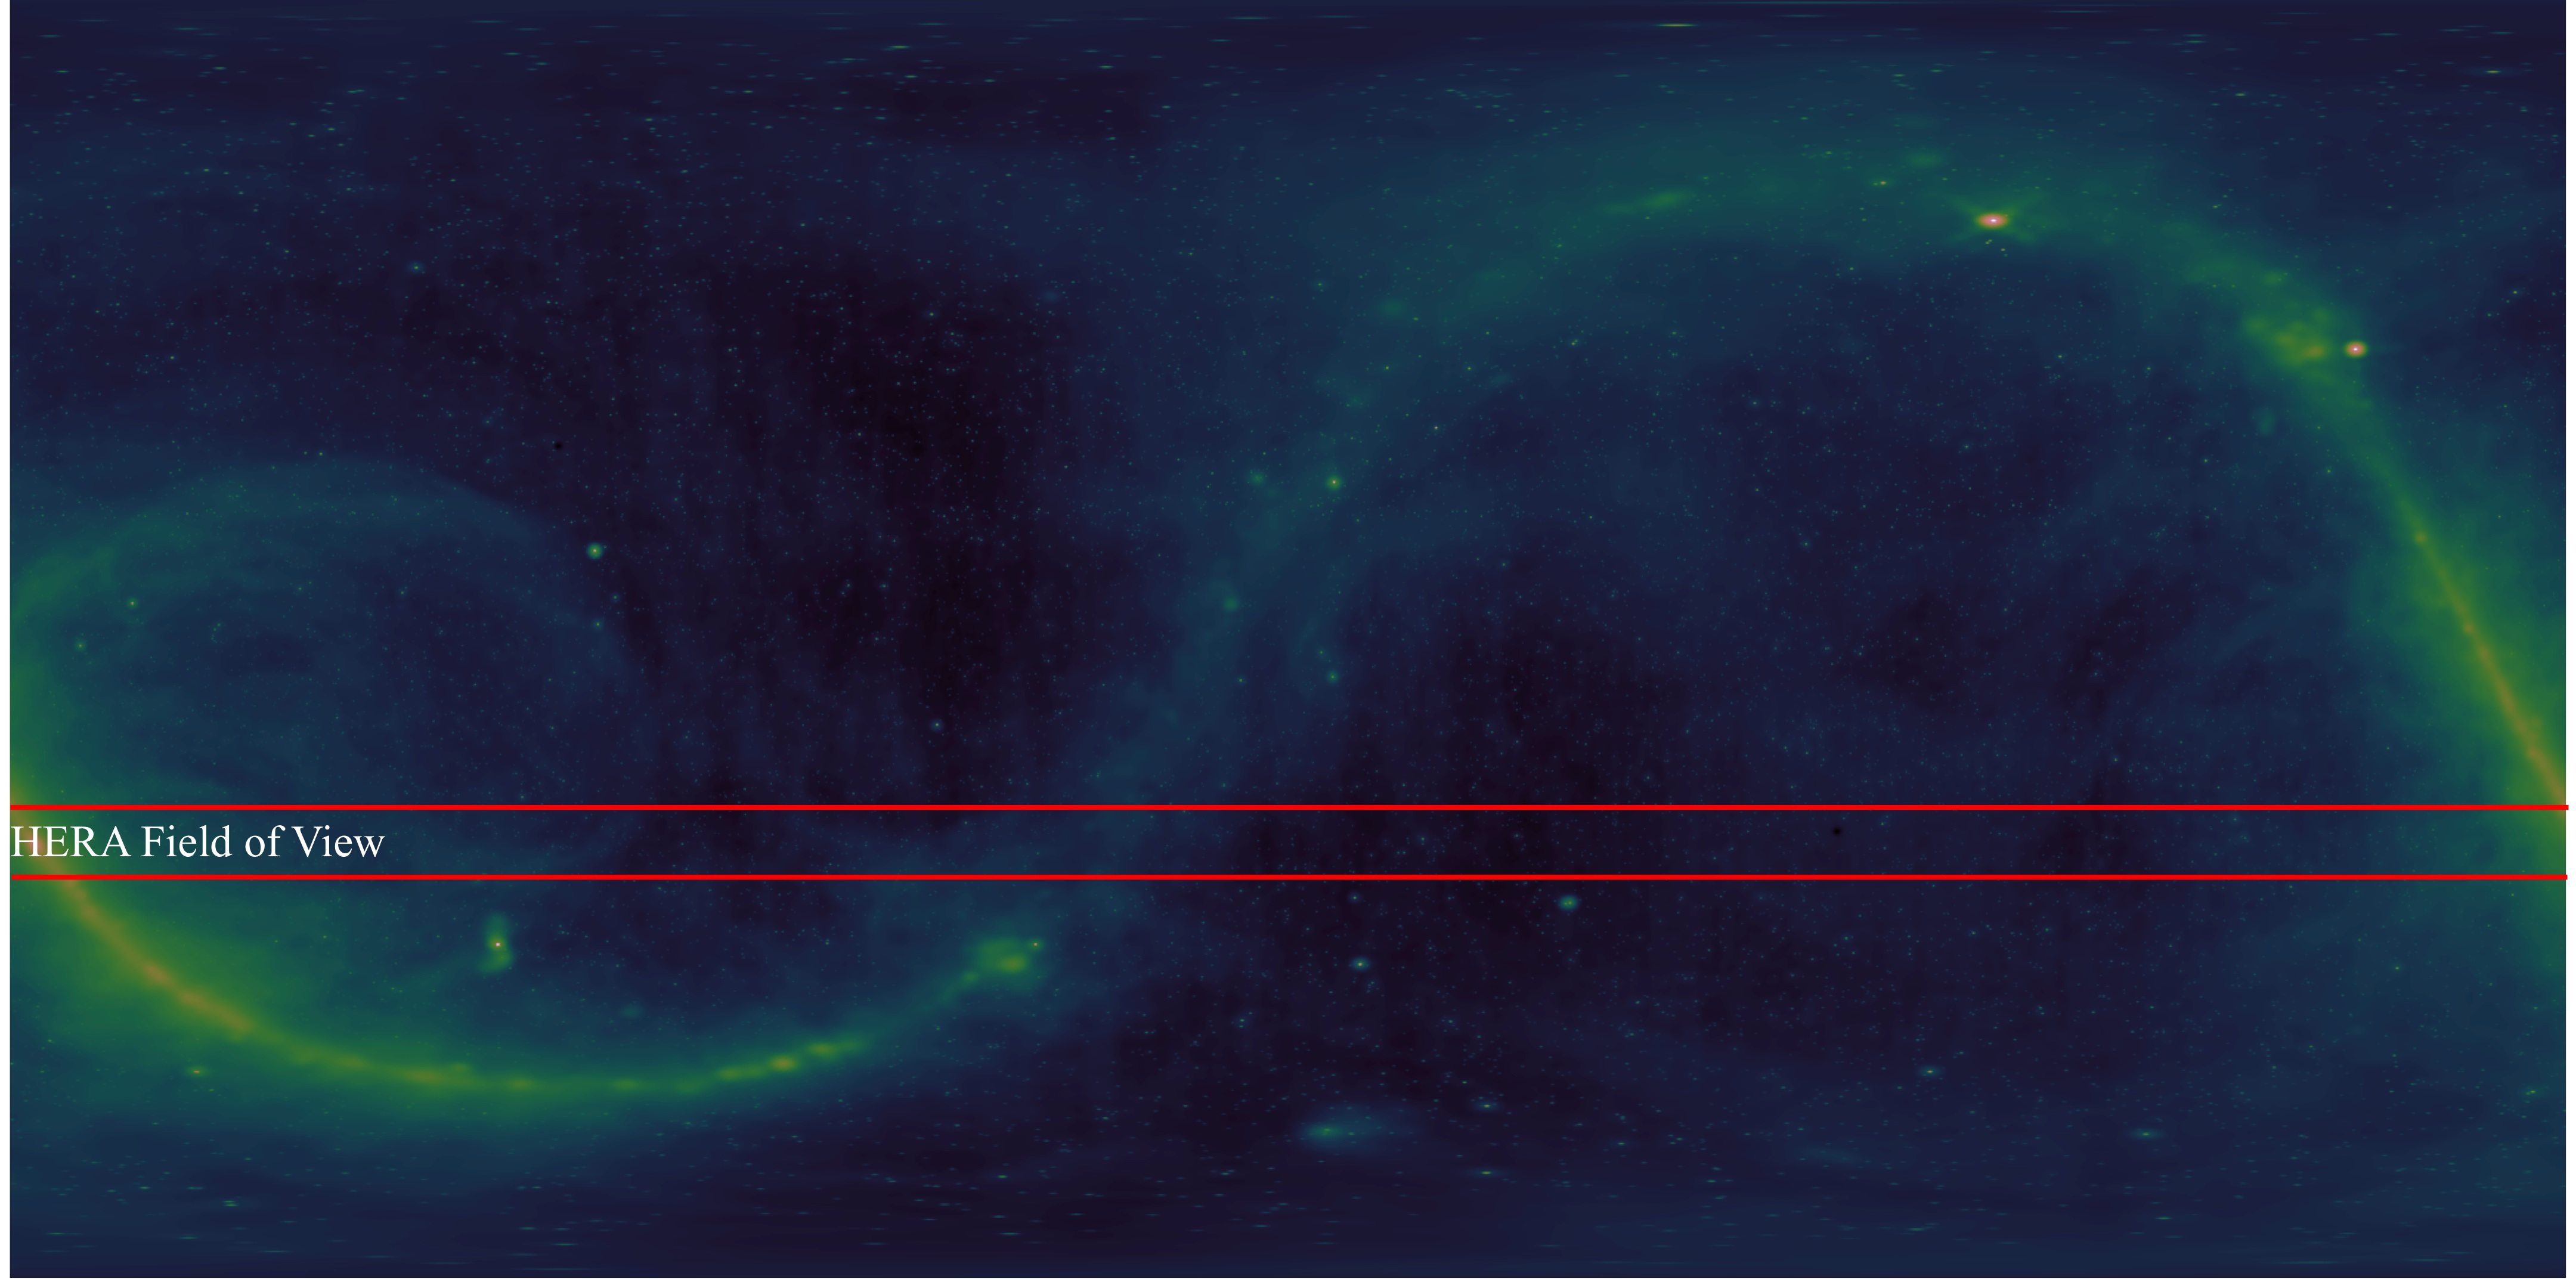
\includegraphics[width=\textwidth]{plots/Imaging/HERA_FoV.jpg}
% XXX ARP: this figure is way to big.  not sure if it should be in (not enough added information)
\caption{The HERA stripe.  At 150MHz ($z=8.5$) the HERA field of view is 8\arcdeg.  With a nearly completely sampled aperture over 300m across, HERA will have the collecting area of Arecibo but with 500x the survey speed. Each night it will drift scan 2600 square degrees for a survey volume of 50 $Gpc^3$.  The stripe includes the GOODs south field, one of the best studied regions of sky. \label{fig:HERA_FoV}}
\end{figure}

With a resolution of 60Mpc and survey area of 1 Gpc$^2$ in a single field of view HERA images will probe structure on scales well beyond any deep, high redshift field contemplated. For comparison, note that the entire Great Observatories Origins Deep Survey (GOODS), where 40\% of all objects at $z > 6$ have been found, is only (30Mpc ) 15{\arcmin } across. Using deep HERA images it will be possible to make targeted observations of early galaxies known to be in the center of large scale bubbles, directly observe clouds responsible for Ly$\alpha$ absorption, and correlate large scale intensity surveys.


 
\begin{figure}[t]\centering
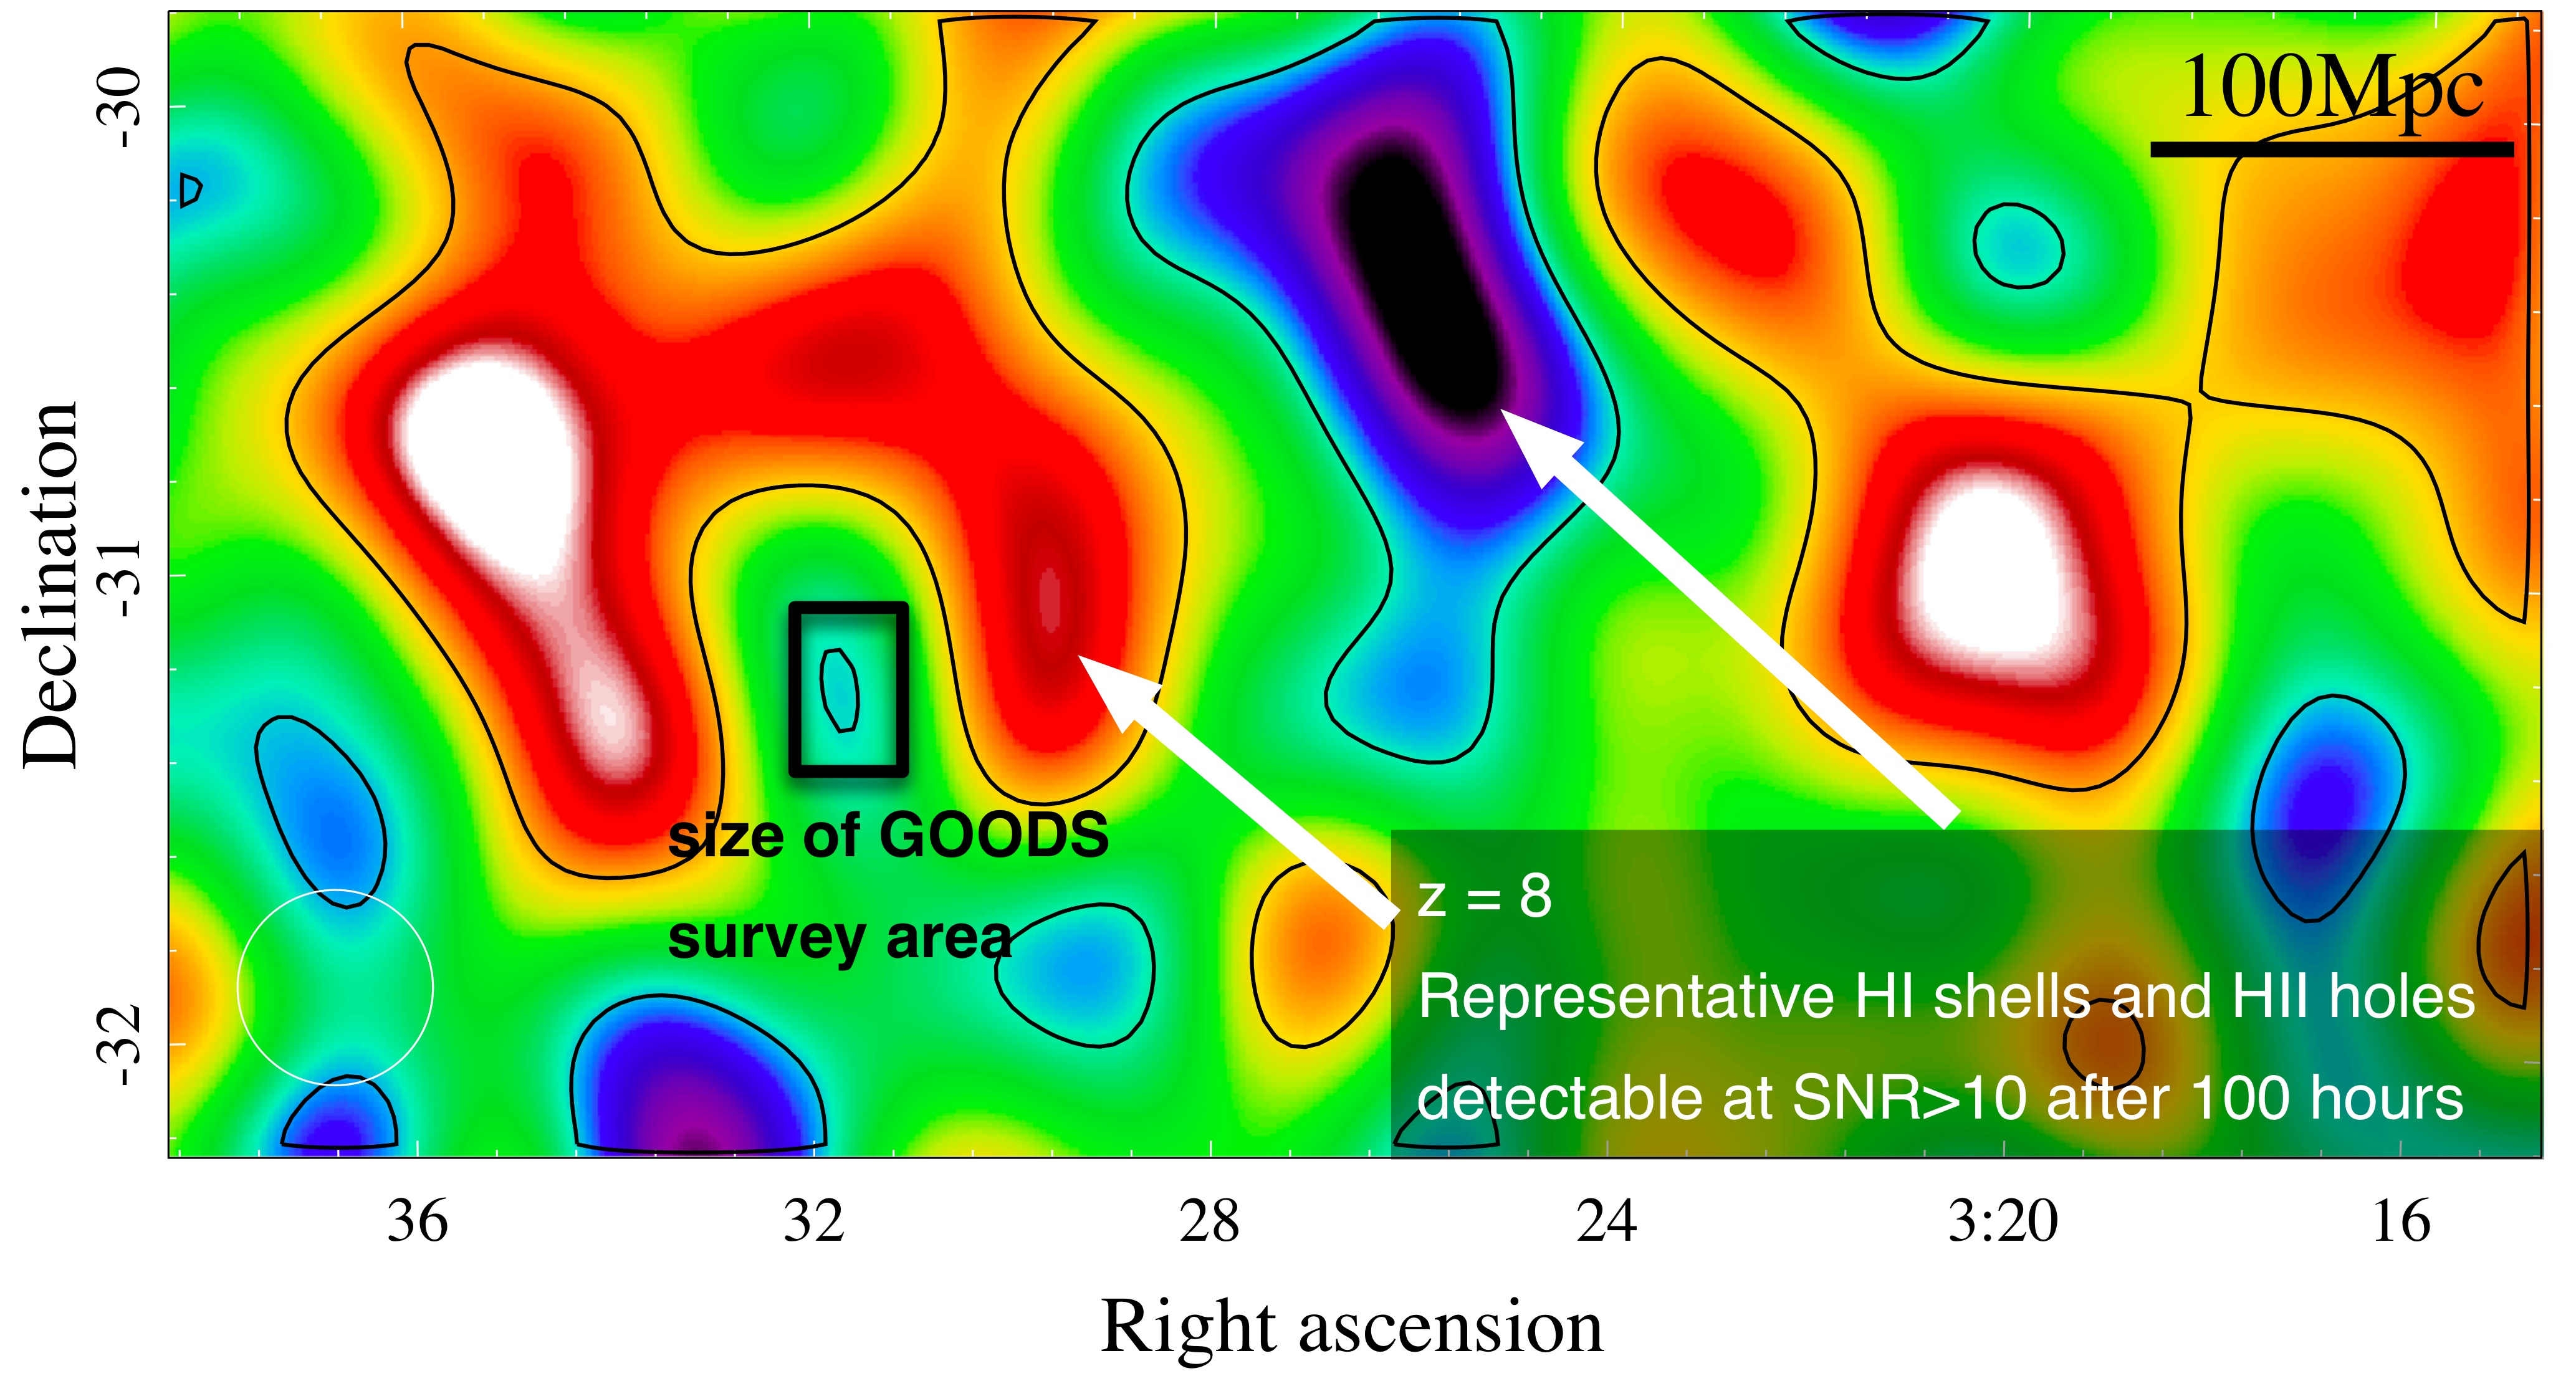
\includegraphics[width=\textwidth]{plots/Imaging/HERA_331_z8_SNR_annotated.jpg}
\caption{\small
With sensitivity highly concentrated at the largest scales, HERA is capable of directly imaging HI during reionization.  Shown here is a simulation of EoR emission (McQuinn 2009) as imaged by HERA with noise equivalent to 100 hours of observation and bandwidth equivalent to the moderate foreground model. %XXX are we using the language of pober et al? 
Contours enclose regions with signal to noise above 10.  The regions detected on scales of $\sim$100 Mpc are bracket the size scales probed by deep galaxy surveys (cf. the GOODs-South survey volume where 40\% of all galaxies above redshift 7 have been detected.)  The GOODs field itself is located within the HERA stripe, just 3 degrees outside of the image shown here.
\label{fig:imaging}}
\end{figure}    

\subsubsection{Imaging as a probe of non-gaussianity}
\emph{a) Imaging as a probe of non-Gaussianity and topology of reionization (Fig from Watkinson \& Pritchard)
[Not sure if this belongs here, should discuss: b) Bayesian imaging (Figs from Paul Sutter).  
Perhaps a broader impact on the radio community too?]}
% Morales, Tegmark

\subsubsection{Early IGM heating}
\emph{v. Approaching Dark ages (z=20 to 30): early Xray heating? other (Fig - Liu models)}
% Liu, Dillon, Hewitt
\begin{figure}[t]\centering
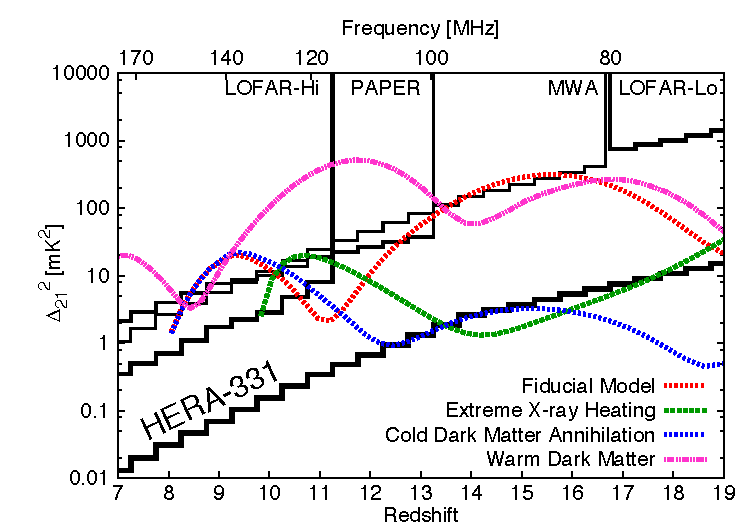
\includegraphics{plots/Xray/HERA_II_compare_kp1_whoriz_20pt.pdf} 
\caption{\small 
At low frequencies, HERA opens a window to
pre-reionization physics at the end of the Dark Ages. Plotted are power spectrum amplitudes (at $k =
0.15h$~Mpc$^{-1}$) for various IGM heating models \citep{mesinger_et_al2013},
with predicted HERA sensitivities.
}\label{fig:Xray} \end{figure}

With high thermal noise sensitivity throughout the observing band, HERA represents an opportunity to push the redshift frontier of current-generation instruments, extending observations to the pre-reionization era in an uninterrupted way.  Doing so will allow a measurement of an earlier peak in the $21\,\textrm{cm}$ power spectrum, corresponding to an era of IGM heating from various X-ray sources.  Theoretical expectations span a wide range of possible scenarios for IGM heating, and Figure \ref{fig:Xray} shows several that were examined in \cite{mesinger_et_al2013}, with HERA's sensitivity overlaid.  It is clear that HERA possesses the sensitivity to easily detect and distinguish between these possibilities, placing the first observational constraints on the pre-reionization epoch, including possible bounds on exotic physics such as dark matter annihilation.


vi. 21cm forest: perhaps a paragraph on possibilities of small scale structure, if we can find radio galaxy? (Fig) 
% Carilli, Furlanetto -- Forget it.  Too much explanation needed. 

\subsubsection{Cross-correlation Science}
%vii. Cross-correlation science: 

perhaps montage Fig showing HI(Tb), galaxies, dark matter... at given epoch
\cite{lidz11}
% Aguirre, Tegmark

a. Provide environmental context for ALMA/JWST 1st galaxy studies

b. CMB pol 

c. CO/CII IM: optimistic or wrong timescale?
  
d. note: xcorr further mitigates continuum systematics

e. Anscillary science with PAPER 128: transients, solar 
% de Boer

%\subsection{Where we are right now: PAPER, MWA}  % 2 pages
\section{Foregrounds \& Lessons Learned from PAPER and MWA} 
% ARP: I think i prefer how the preproposal fused all of this in a section.  Very hard to talk about only 1 aspect at a time

The key challenge of 21-cm cosmological reionization experiments is 
balancing the stringent sensitivity requirements needed to detect the faint 21cm reionization signal
with the need to suppress
foregrounds (see Figure~\ref{fig:twoFGViews}, left) that are $\sim$5 orders of magnitude brighter.
A major breakthrough in 21-cm cosmology---what enables us to propose HERA now---is 
the discovery of how 
instrumentation and analysis can exploit the 
spectral smoothness of foregrounds
to open up an `EoR Window'.  
% XXX better phrase for "EoR window"?
These advances have been used to suppress foreground emission by 4
orders of magnitude in PAPER observations,
with results that begin ruling out certain reionization scenarios
\citep{parsons_et_al2013}.

Observations for 21-cm cosmology experiments are best understood in
Fourier space.  Because the \HI emission is a
narrow spectral line, the observed frequency of the emission can be mapped to
redshift or line-of-sight distance to provide an observed volume $\{x,y,z\}$ in
comoving Mpc. This observed volume is Fourier transformed into a 3D
wavenumber cube $\k\equiv\{k_{x}, k_{y}, k_{z}\}$. For graphical simplicity, the angular
wavenumbers are typically averaged ($\{k_{x},k_{y}\}\rightarrow\kperp$) to
produce line-of-sight wavenumber $\kpar$ vs.\ angular $\kperp$. 
%Interferometric measurements are of the angular Fourier modes in many
%frequency channels (visibilities), so in the absence of widefield effects only
%a Fourier transform in the frequency direction and a coordinate mapping is
%needed to obtain the 3D $\{k_{x}, k_{y}, k_{z}\}$ measurements
%\citep{morales_hewitt2004}.) 
The expected statistical isotropy of the signal allows measurements in $\k$-space to be
squared and averaged in shells to produce the spherical power spectrum
shown in Figure \ref{fig:eor_pspec}.

Recently, the MWA and PAPER teams have made substantial advances in understanding how smooth-spectrum 
foreground emission interacts with the instrument to produce the EoR Window.
Through a concerted theoretical and observational campaign
\citep{morales_et_al2012,parsons_et_al2012b,vedantham_2012,Datta_2010,hazelton_et_al2013,pober_et_al2013,parsons_et_al2013,dillon_et_al2013b}
we now understand that foreground contamination can be confined to a `wedge' in
$\kpar$ vs.\ $\kperp$, as demonstrated by the PAPER observations in the
righthand panel of of Figure \ref{fig:twoFGViews}. This wedge is the result of
the smooth spectrum foregrounds 
%XXX SF: I would make this more obvious.  I recommend replacing this sentence with something like (with my naive understanding): "This sharp division occurs because foregrounds have smooth spectra (which cause the sources to manifest at small $\kpar$), some of which is projected into the transverse direction ($\kperp$) through the instrument's well-understood chromatic properties."
(low $\kpar$) interacting with the inherent
chromaticity of an interferometer. 
This leaves the region above the wedge free from 
foreground emission---a window through which we can observe the EoR.

Observations with PAPER and the MWA have confirmed the presence of the EoR Window
\citep{pober_et_al2013,dillon_et_al2013b}, and recent PAPER observations
have measured the foreground suppression within it
to be at least 4 orders of magnitude 
(8 in mK$^2$;
\citealt{parsons_et_al2013}).
This is a major advance---we can
suppress foregrounds and we understand the instrumental and analysis
characteristics needed to perform the EoR measurement.

Understanding the origin of the EoR Window has enabled us to improve our
instrumentation and analysis 
tools to precisely measure the 21-cm
signal. HERA's antennas (see \S \ref{PDsec}) are optimized 
to yield $\sim$20
times the sensitivity per element (relative to PAPER) without substantially degrading
foreground isolation,
and we have developed new imaging and
analysis techniques to suppress polarized source contamination to below the EoR
signal within the window \citep{bernardi_2013_trunc,moore_et_al2013}.
Together, these advances provide the necessary foreground suppression and
a game-changing level of sensitivity at a fraction of the
cost anticipated in the HERA roadmap.

\begin{figure}[t] \centering
%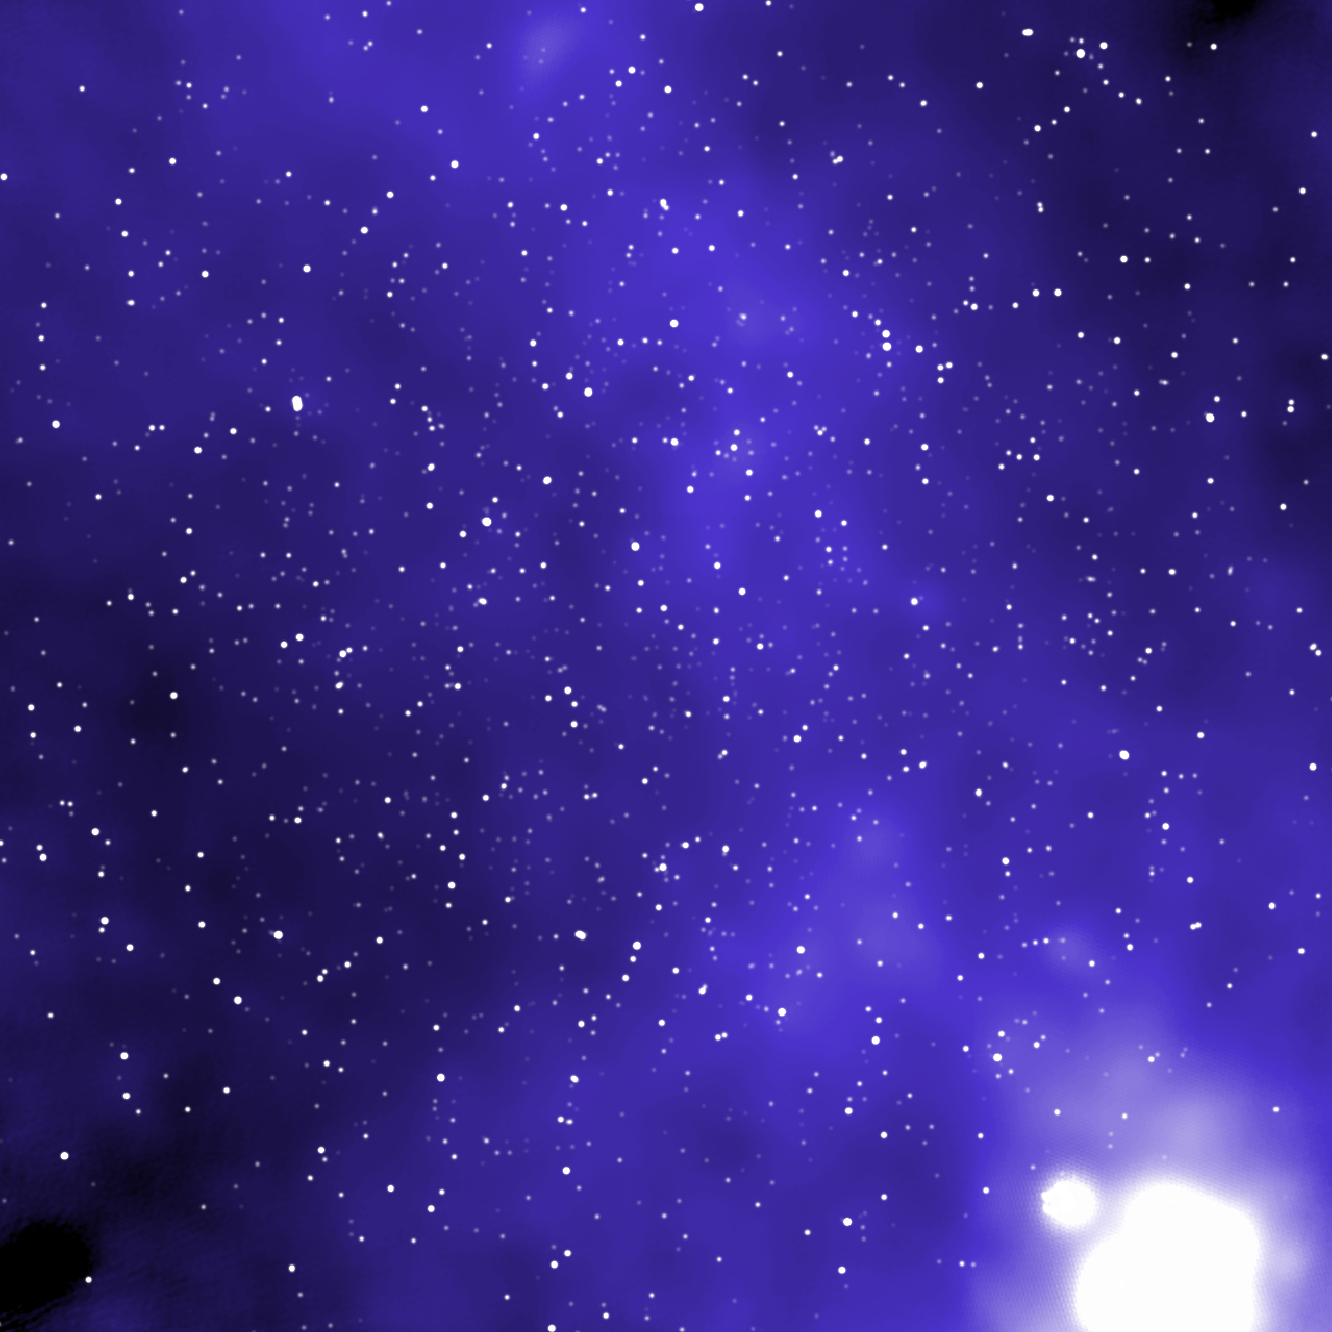
\includegraphics[width=6.5in]{plots/MWApretty.png} 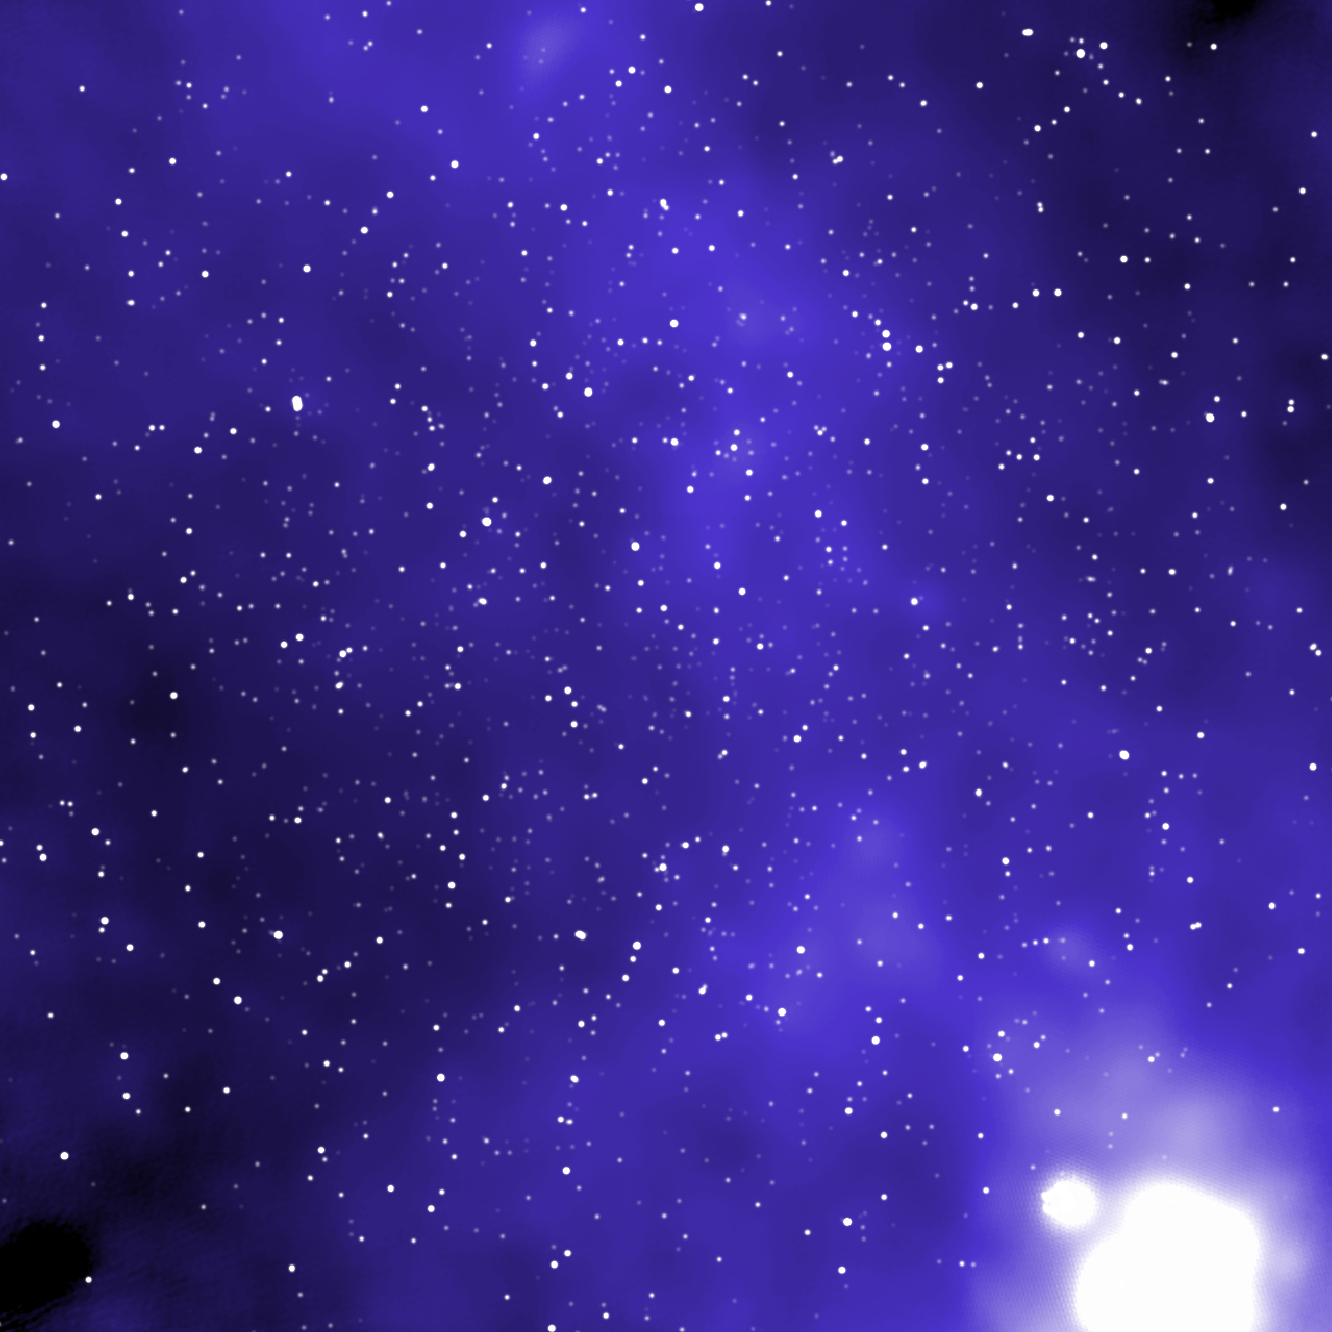
\includegraphics[width=3.6
%in]{plots/MWApretty.png}
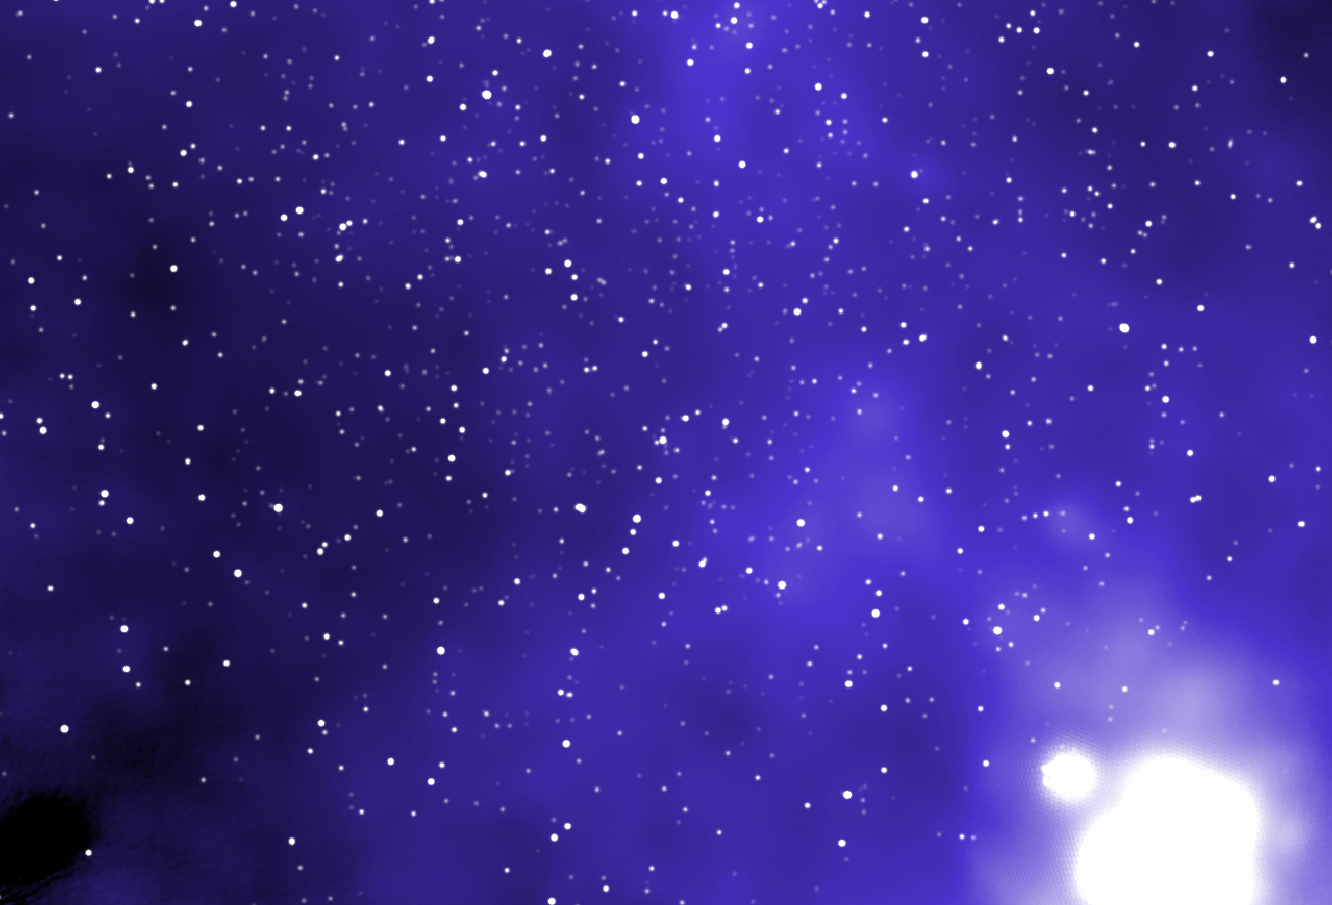
\includegraphics[height=2.3in]{plots/MWApretty_crop.png} 
%\includegraphics[width=2.4 in]{plots/wedge_tall.png}
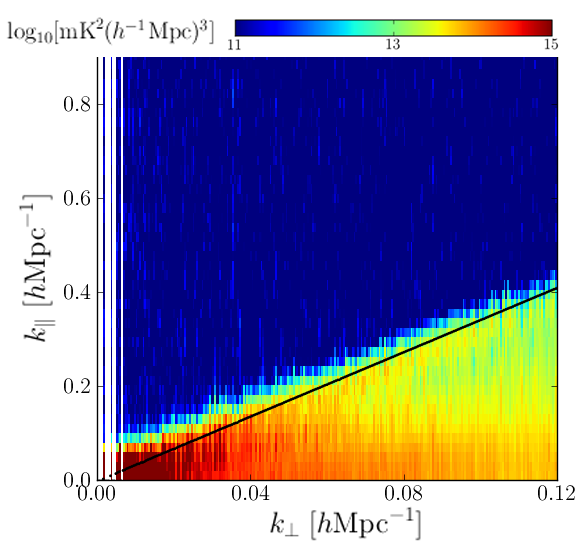
\includegraphics[height=2.3in]{plots/wedge_tall_wide.png} \caption{\small Left:
Foregrounds imaged on the MWA using FHD software.
This image spans $\sim$$30^{\circ}$ and
includes point-source and diffuse emission (the Vela and Puppis SNRs are in the
bottom-right). Imaging methods provide a key capability for reducing
polarization leakage and foreground systematics.  
Right: Foreground contamination in line-of-sight $\kpar$ vs.\ angular $\kperp$
as observed using PAPER \citep{pober_et_al2013}.
Foregrounds are bright within a ``wedge" (lower right) and then fall 
precipitously in the ``EoR window" (blue/black 
region), where measurements are thermal-noise limited.  The wedge's location can 
be estimated analytically (solid black line), but the foregrounds leak out by a margin 
dictated by the chromatic properties of both the foregrounds and the instrument.
%Bright foregrounds occupy
%a wedge (lower right) that extends beyond a fundamental analytic limit
%(solid black) by a margin dictated by the chromatic properties of the foregrounds
%and the instrument, and then falls precipitously
%in the EoR Window (blue
%region), where measurements are currently thermal noise limited. 
This insight has led to the
first meaningful constraints on EoR via 21-cm emission
\citep{parsons_et_al2013}.
}\label{fig:twoFGViews} \end{figure}



%i. describe arrays, state design driven by new understandings as delineated below (Fig)
% ARP: check, above % Parsons, Bowman

%ii. Using new techniqes, current best limits  (Fig)
% ARP: check, above % Parsons, Morales

iii. what will happen in next 2 years: hopefully detection, but no more

%iv. LOFAR/MWA/PAPER 
% Carilli
% XXX ARP: I think paragraph below should really emphasize concrete limitations of 
% current experiments, and describe how HERA blows this wide open
Three reionization path-finder array experiments are currently
operational: LOFAR, MWA and PAPER. All three are designed to have the
sensitivity to make the first statistical detection of the neutral
IGM. However, the HI line experiment is very challenging due to
foreground continuum emission some four orders of magnitude brighter
than the expected line signal.  The three experiments offer very
significant complementarity, with different intrinsic systematics and
different approaches to foreground mitigation. We emphasize that, for
such an important discovery, multiple approaches are critical in order
to check and verify any claimed (likely low S/N) detection amidst the
substantial systematic uncertainties. The first detection of
the neutral IGM is not the end of reionization studies, just the 
beginning. Recall that some four decades separated the first detection
of the CMB from the first statistical characterization. 


iv. HERA II: 'gauranteed' detection, full characterization, dark ages, imaging
% Aguirre

v. Move 'analysis' stuff here?


\section{Challenges} % 2 pages

\subsection{Foregrounds}  % 1.5pages
% Parsons, Morales


i. relative intensities (Fig: Continuum from MWA)

ii. Details on Delay Spectrum approach

a. key: 3D k-space: show wedge and discuss. chromatic sidelobes with characteristic freq scale 
set by baseline length

b. analysis focuses on line-of-sight PS dimension

c. work in EoR window.  different window levels, depending on effective horizon

d. drives design to redundant array: helps calibration, add spectra coherently

e. dictates geometry of antenna elements and other RF stuff. avoid standing waves of given length. 

f. area: drives sensitivity as used in section 2

g. some words about why compact, hex array 

\subsection{Other Challenges} % 0.5 pages

i. Interference: Karoo RFI plots  FIG 
% Jacobs

i. Polarization 
% Moore, Aguirre
% XXX ARP: I'm worried about this section.  In my mind, this is the one risk we
% haven't truly retired yet.  We need to tread very carefuly if we bring this
% up in depth.

D. Ionosphere: 

i. short baselines and narrowish FoV

ii. direction dependent gains?


\section{HERA design and project} % 8 pages

\subsection{Lessons learned recap} % 0.5 page
The HERA collaboration has made significant progress on multiple approaches in dealing with
foregrounds.
Based on a ``delay-spectrum'' understanding of
the mechanism for how instrumental responses modulate foregrounds on
spectral scales of cosmological interest \citep{parsons_et_al2012b},
PAPER has optimized its instrument to focus on regions in Fourier
space that have weak coupling to foregrounds caused by the
interferometer.  These regions are determined both by chromatic
instrumental responses and by the inherent frequency structure of the
foregrounds.  An `EoR window' has been identified in the Fourier
(wavenumber) space of spectral and angular power spectra that is
inherently free of continuum emission, without explicit continuum
subtraction in either the image or spectral domain \citep{pober_et_al2013,morales_et_al2012,Datta_2010}
This window allows for continuum
`avoidance' rather than subtraction. Observations based on this new
approach have already demonstrated that the extremely stringent level
of foreground suppression needed to access the 21cm signal is largely
in hand (as shown in Figure \ref{fig:pk_k3pk}), with upper limits
that are beginning to rule out cold reionization scenarios.

HERA-331 proposal targets a 331-element array that incorporates
our proven foreground avoidance techniques while improving
dramatically the sensitivity relative to current experiments.  With a
new understanding of how antenna size and separation affect
sensitivity and foreground isolation, it has become evident a revision
of the PAPER antenna design can yield up to 20 times the sensitivity
per element without substantially degrading foreground isolation.
Where PAPER's elements lack collecting area and are smaller than
strictly required for foreground isolation, and the majority of MWA
and LOFAR elements are spaced too widely to avoid foregrounds,
HERA-331 employs an extremely compact array of 14-m parabolic dishes
with PAPER-style dipole feeds (see Figure \ref{fig:hera_dish}.  The
short (4.5m) focal height of these dishes is central to limiting the
path length of reflections whose time-delay gives rise to chromatic
instrumental systematics.

% AAARRGGHH!
\begin{figure}[!ht]
\centering
	\begin{subfigure}[b]{0.46\textwidth}
		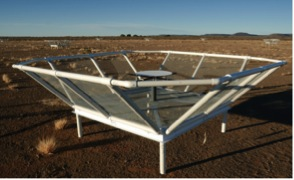
\includegraphics[width=\textwidth]{plots/paper_element.jpg}
		\caption{The PAPER element (provides a clean instrumental response as a function
		of frequency \citep{parsons_et_al2010,parsons_et_al2012b}, which is crucial to
		the foreground isolation shown in Figure \ref{fig:eor_pspec}.}
	\end{subfigure}
	\quad
	\begin{subfigure}[b]{0.46\textwidth}
		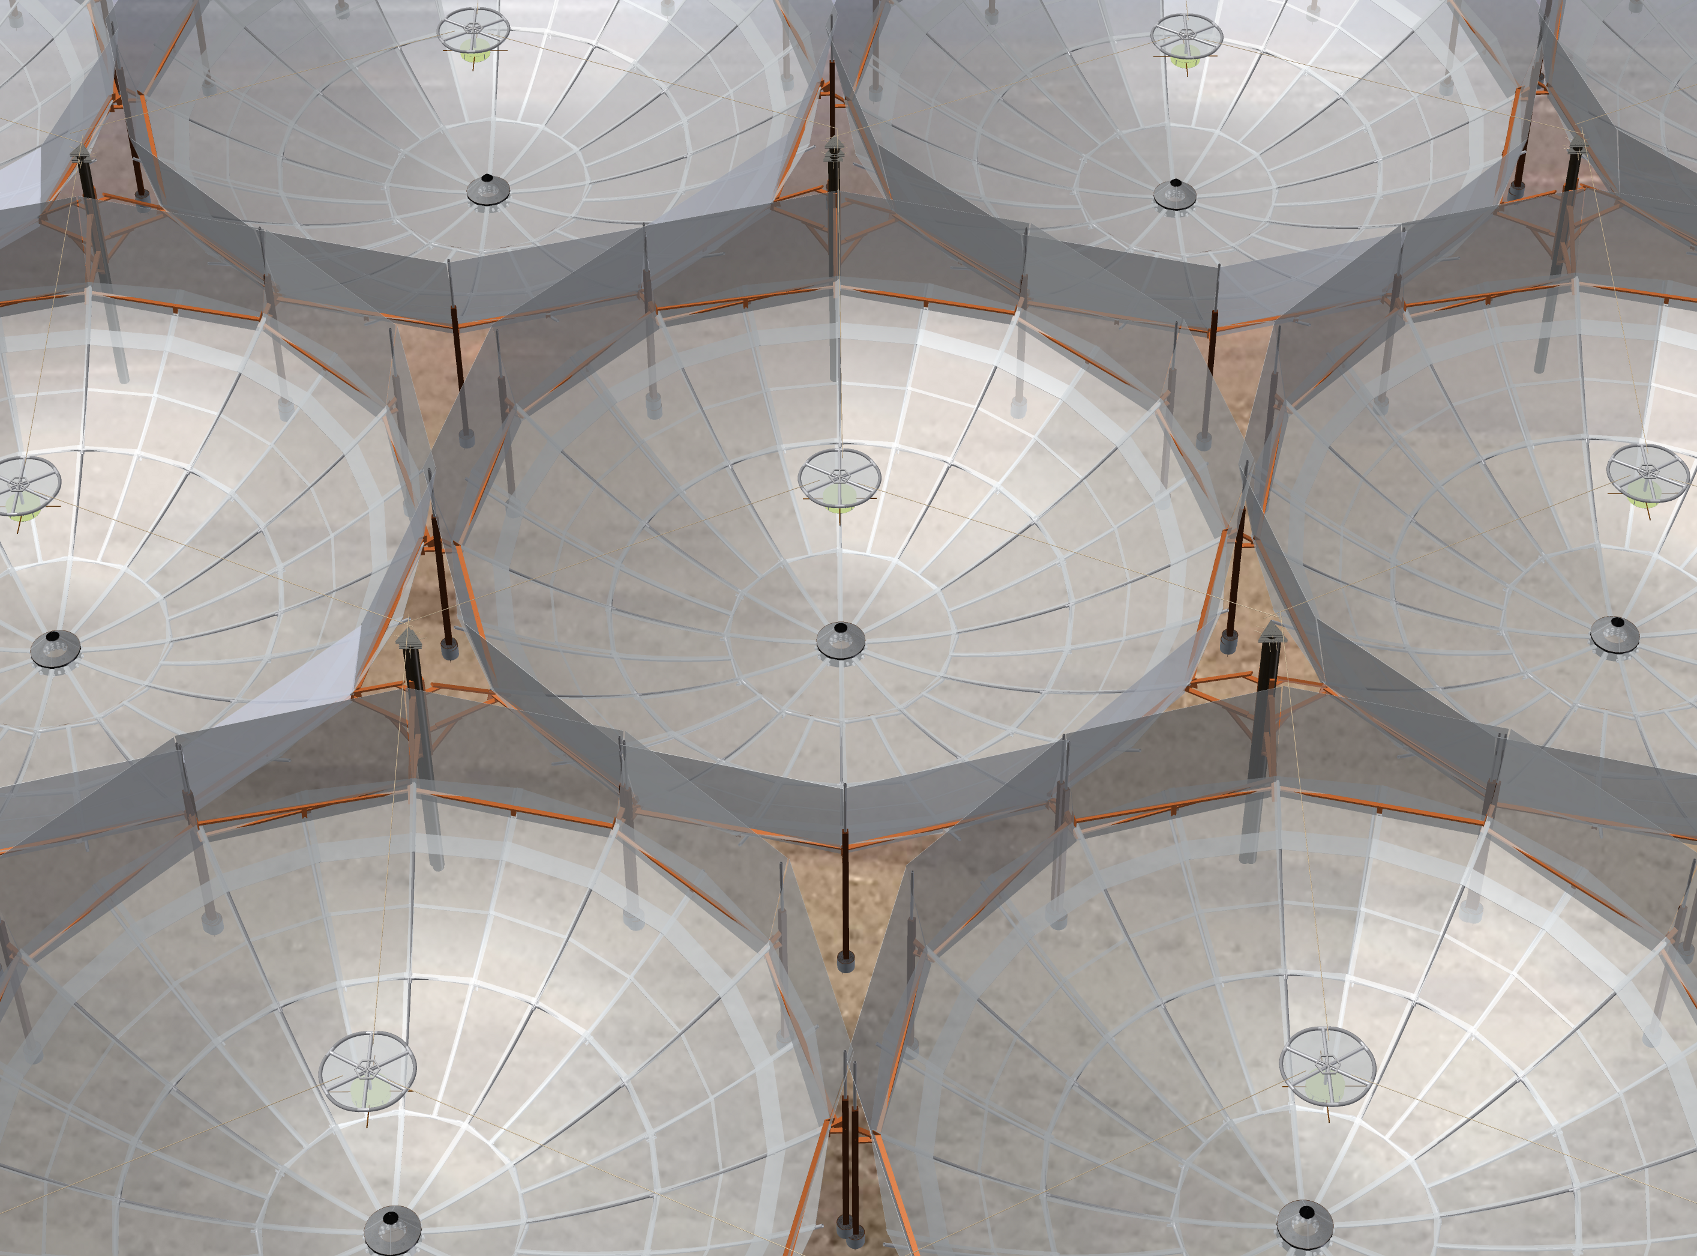
\includegraphics[height=1.75in]{plots/hera_dish.png}
		\caption{A 14m dish designed around the feed dramatically improves sensitivity while
		constraining the path length and amplitude of reflections to ensure that foreground 
		isolation is not substantially degraded.}
	\end{subfigure}
\caption{PAPER and HERA elements}
\label{fig:hera_dish}
\end{figure}

The size of HERA-331 dishes optimizes cost for a fixed sensitivity and
level of foreground isolation.  The associated reduction in the number
of antenna elements to achieve a given collecting area, combined with
the fact that these dishes have no moving parts, are built from
inexpensive materials, and follow a simple construction that can be
contracted locally, makes the cost of building HERA-331 substantially
cheaper than was anticipated in the roadmap submitted to \nwnh\ for this
stage of the program.   

HERA leverages the technical heritage of PAPER, MWA and of CASPER\footnote{Collaboration for Astronomical
Signal Processing and Electronics Research, a Berkeley-initiated worldwide open source community that is
developing boards, firmware and software for the astronomical community} and incorporates a
phased implementation to mitigate against risk.  The system, technology and phased approach is discussed below
in more detail.

\vspace{-0.25in}
\subsection{Instrument Design}
\vspace{-6pt}
\label{InstDes}
The HERA instrument design is very straightforward.  The element
itself is a fixed zenith-pointing 14-meter segmented prime-focus paraboloid with a high screen
to minimize cross-talk between elements (which are spaced 14.3 meters on a
hexagonal grid.   The $f/D$ of
the paraboloid is 0.32, so that the focal length, $f$, is less than 5 meters to meet the 
standing wave specification at the delays of interest of more than 60 dB of attenuation at delays 
greater than 50 ns.


The active feed sends back the entire dual-polarization analog bandwidth on standard
coaxial cable to an aggregation point called a ``node'', which services 
about 15 antennas.  This cable length is kept short (35-m) to keep any standing
wave contamination outside of the delay-space of interest for power spectrum
measurements.  The node amplifies, filters, digitizes and transmits the signal data stream
back to the central processing location (the Karoo Array Processing Building - KAPB).
Figure \ref{fig:blockDiagram} shows a block diagram of the system.

\begin{figure}[h]
\centering
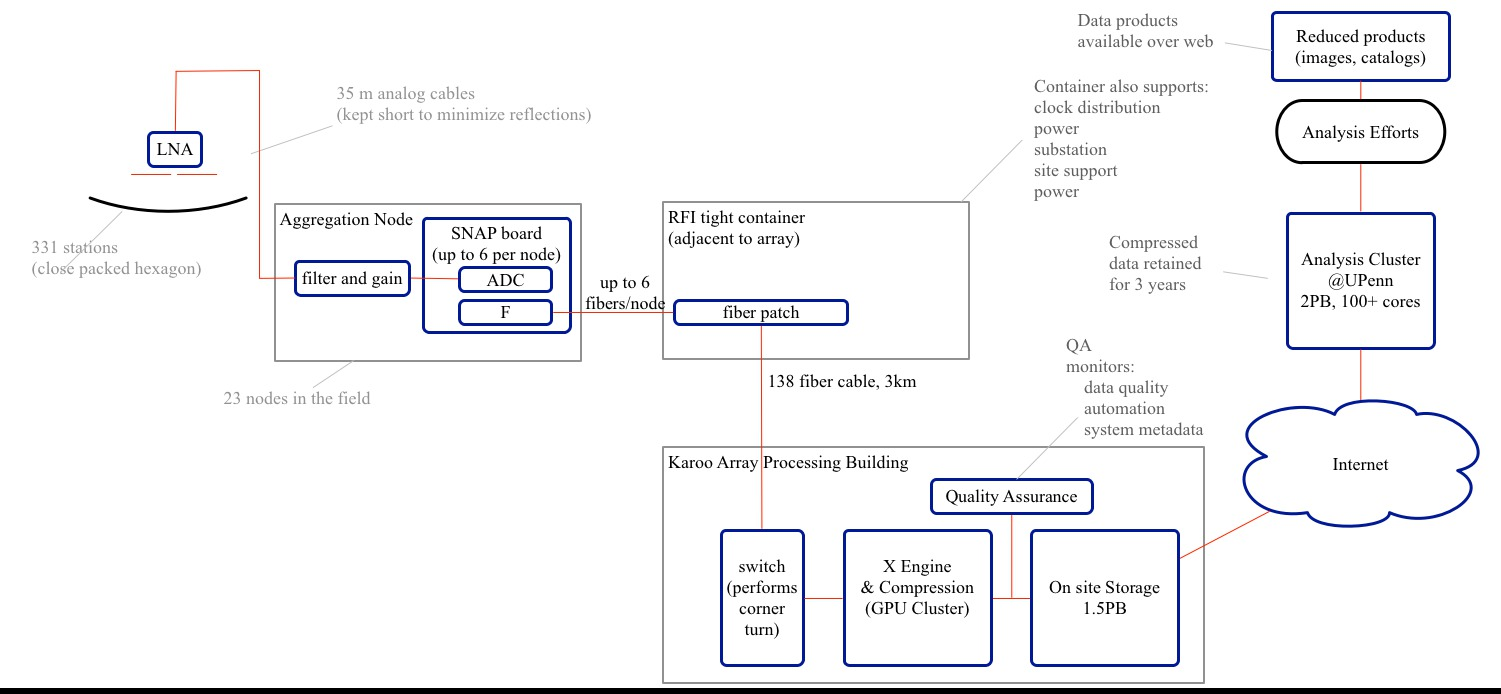
\includegraphics[width=\textwidth]{plots/Engineering/HERA_high_level_block_diagram.jpg}
\caption{Block diagram of the HERA system.}
\label{fig:blockDiagram} 
\end{figure}

\vspace{-0.25in}
\subsubsection{Element and Configuration}
\vspace{-6pt}


The element is a fixed zenith-pointed mount, which dramatically simplifies design and
operation. Cost is a key design constraint for this experiment, which has components
for construction materials, assembly in a remote area, and operation over its
lifetime. As an experiment, the design lifetime is 6 years, which helps constrain
costs relative to a long-lived facility. For a field-deployed instrument, one needs
to define limited well-constrained reference points for accuracy in construction. The
proper installation procedure is therefore critical in construction. The elements are
also nearly abutting one another, which allows for sharing of physical support
infrastructure.

Given the delay-spectrum technique developed for 21-cm EoR science, it is important
to ensure that internal reflections within the antenna structure are at a low enough
level at delay values where the array has sensitivity to the EOR power spectrum. That
is, we don't want reflections that will modulate foregrounds to corrupt scales
corresponding to the desired $\kpar$, scattering foreground power into the EoR
window. Recent work characterizing foregrounds suggests that the spectral structure
of foregrounds observed with baseline separations of $8\lambda \approx 15$m are
well-behaved to current limits \citep{parsons_et_al2013}. This sets the upper limit
for the dish diameter at about 15m. However, this requirement also sets restrictions
on the focal length of the dish since the primary resonances in the dish will be the
standing waves that arise between the primary reflector and the antenna feed, caused
by imperfect impedance matches of the feed electronics and free space, as well as by
the presence of any metallic structure in the area.

Many competing factors set the area of the collecting element. Among them are
sensitivity, cost, minimum baseline, efficiency and delay values of internal
reflections, as just mentioned. Using the derived sensitivity for a redundant array
\citep{parsons_et_al2012a} and a reasonably complete costing model, one can compute
the cost/performance for a fixed sensitivity as a function of diameter. Figure
\ref{fig:nvsd} shows this function normalized to a 14-meter antenna, indicating a
fairly broad minimum extending from about 14 to 22 meters. Arrows indicate the
direction of increasing systematics and delay-space contamination. Within this range,
smaller elements are preferred because of increased field of view and lower
timescales for delay-space contamination arising from reflections.

% AAARRGGHH!
\begin{figure}[h]
	\centering
	\begin{subfigure}[b]{0.46\textwidth}
		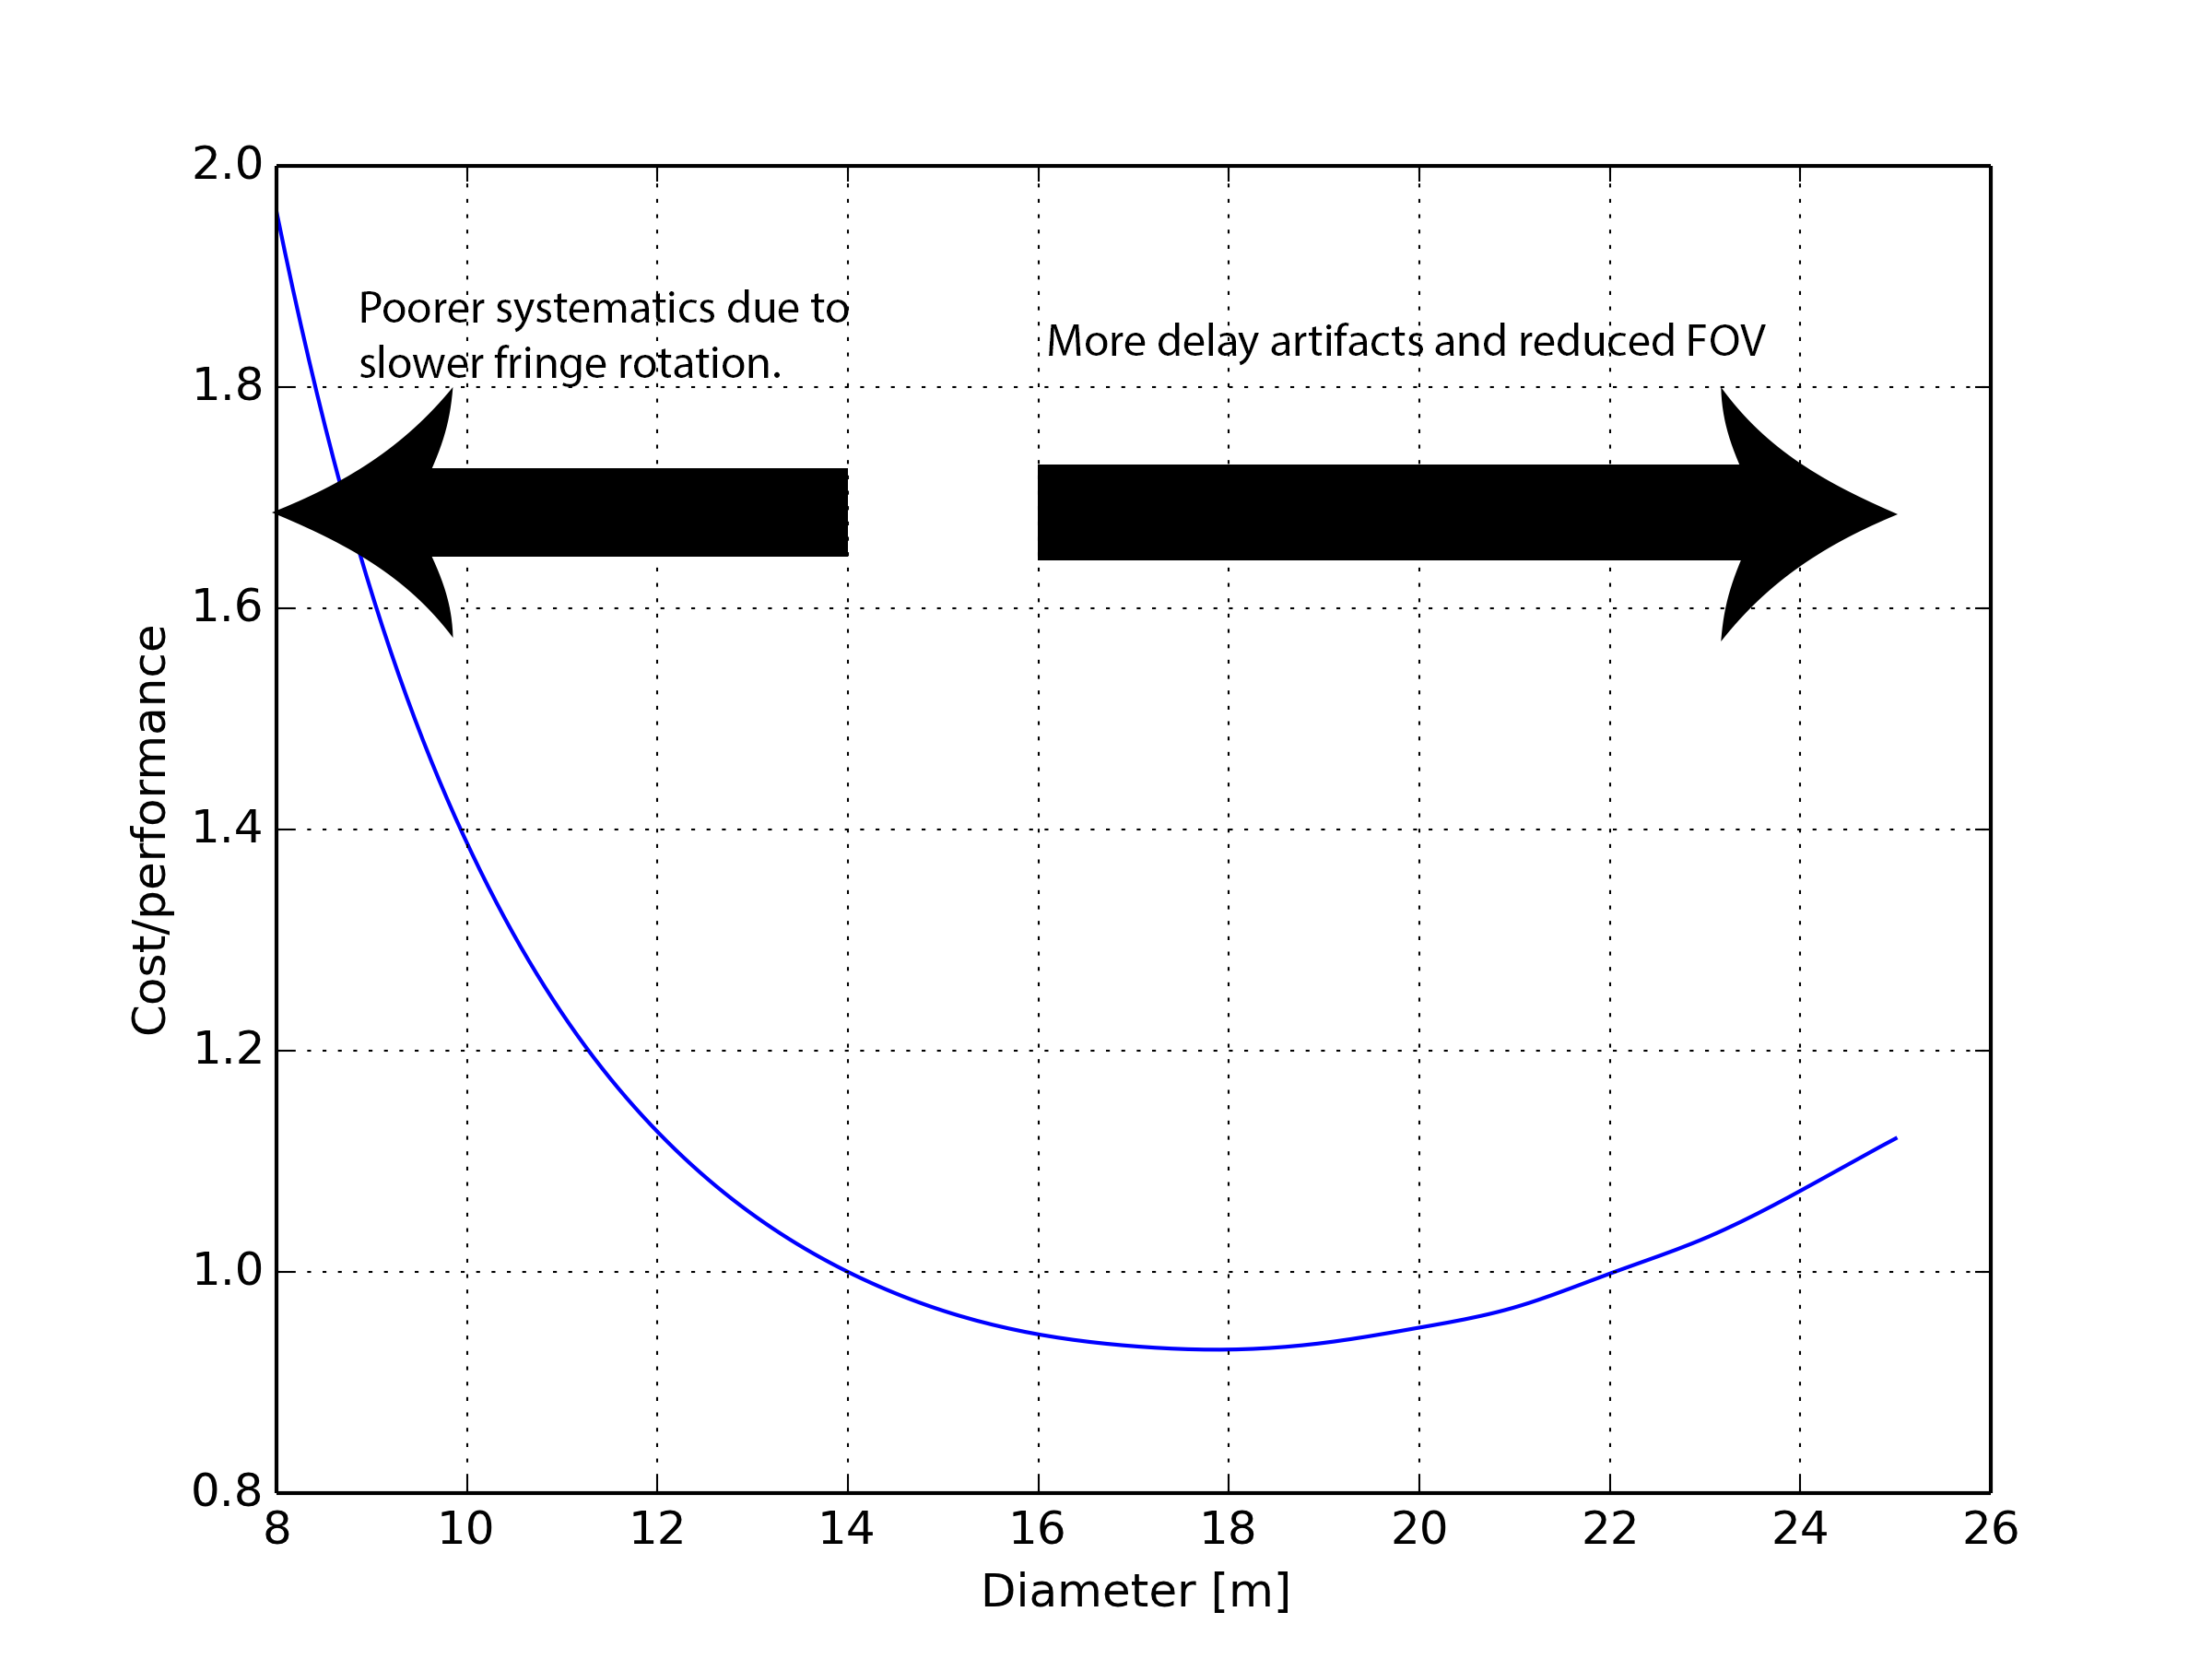
\includegraphics[width=0.9\textwidth]{plots/Engineering/nvsd.png}
		\caption{Costing model for a fixed sensitivity and varying the diameter.   The arrows indicate the regions of 
				increasing systematics and delay-space contamination.}
		\label{fig:nvsd} 
	\end{subfigure}
	\quad
	\begin{subfigure}[b]{0.46\textwidth}
		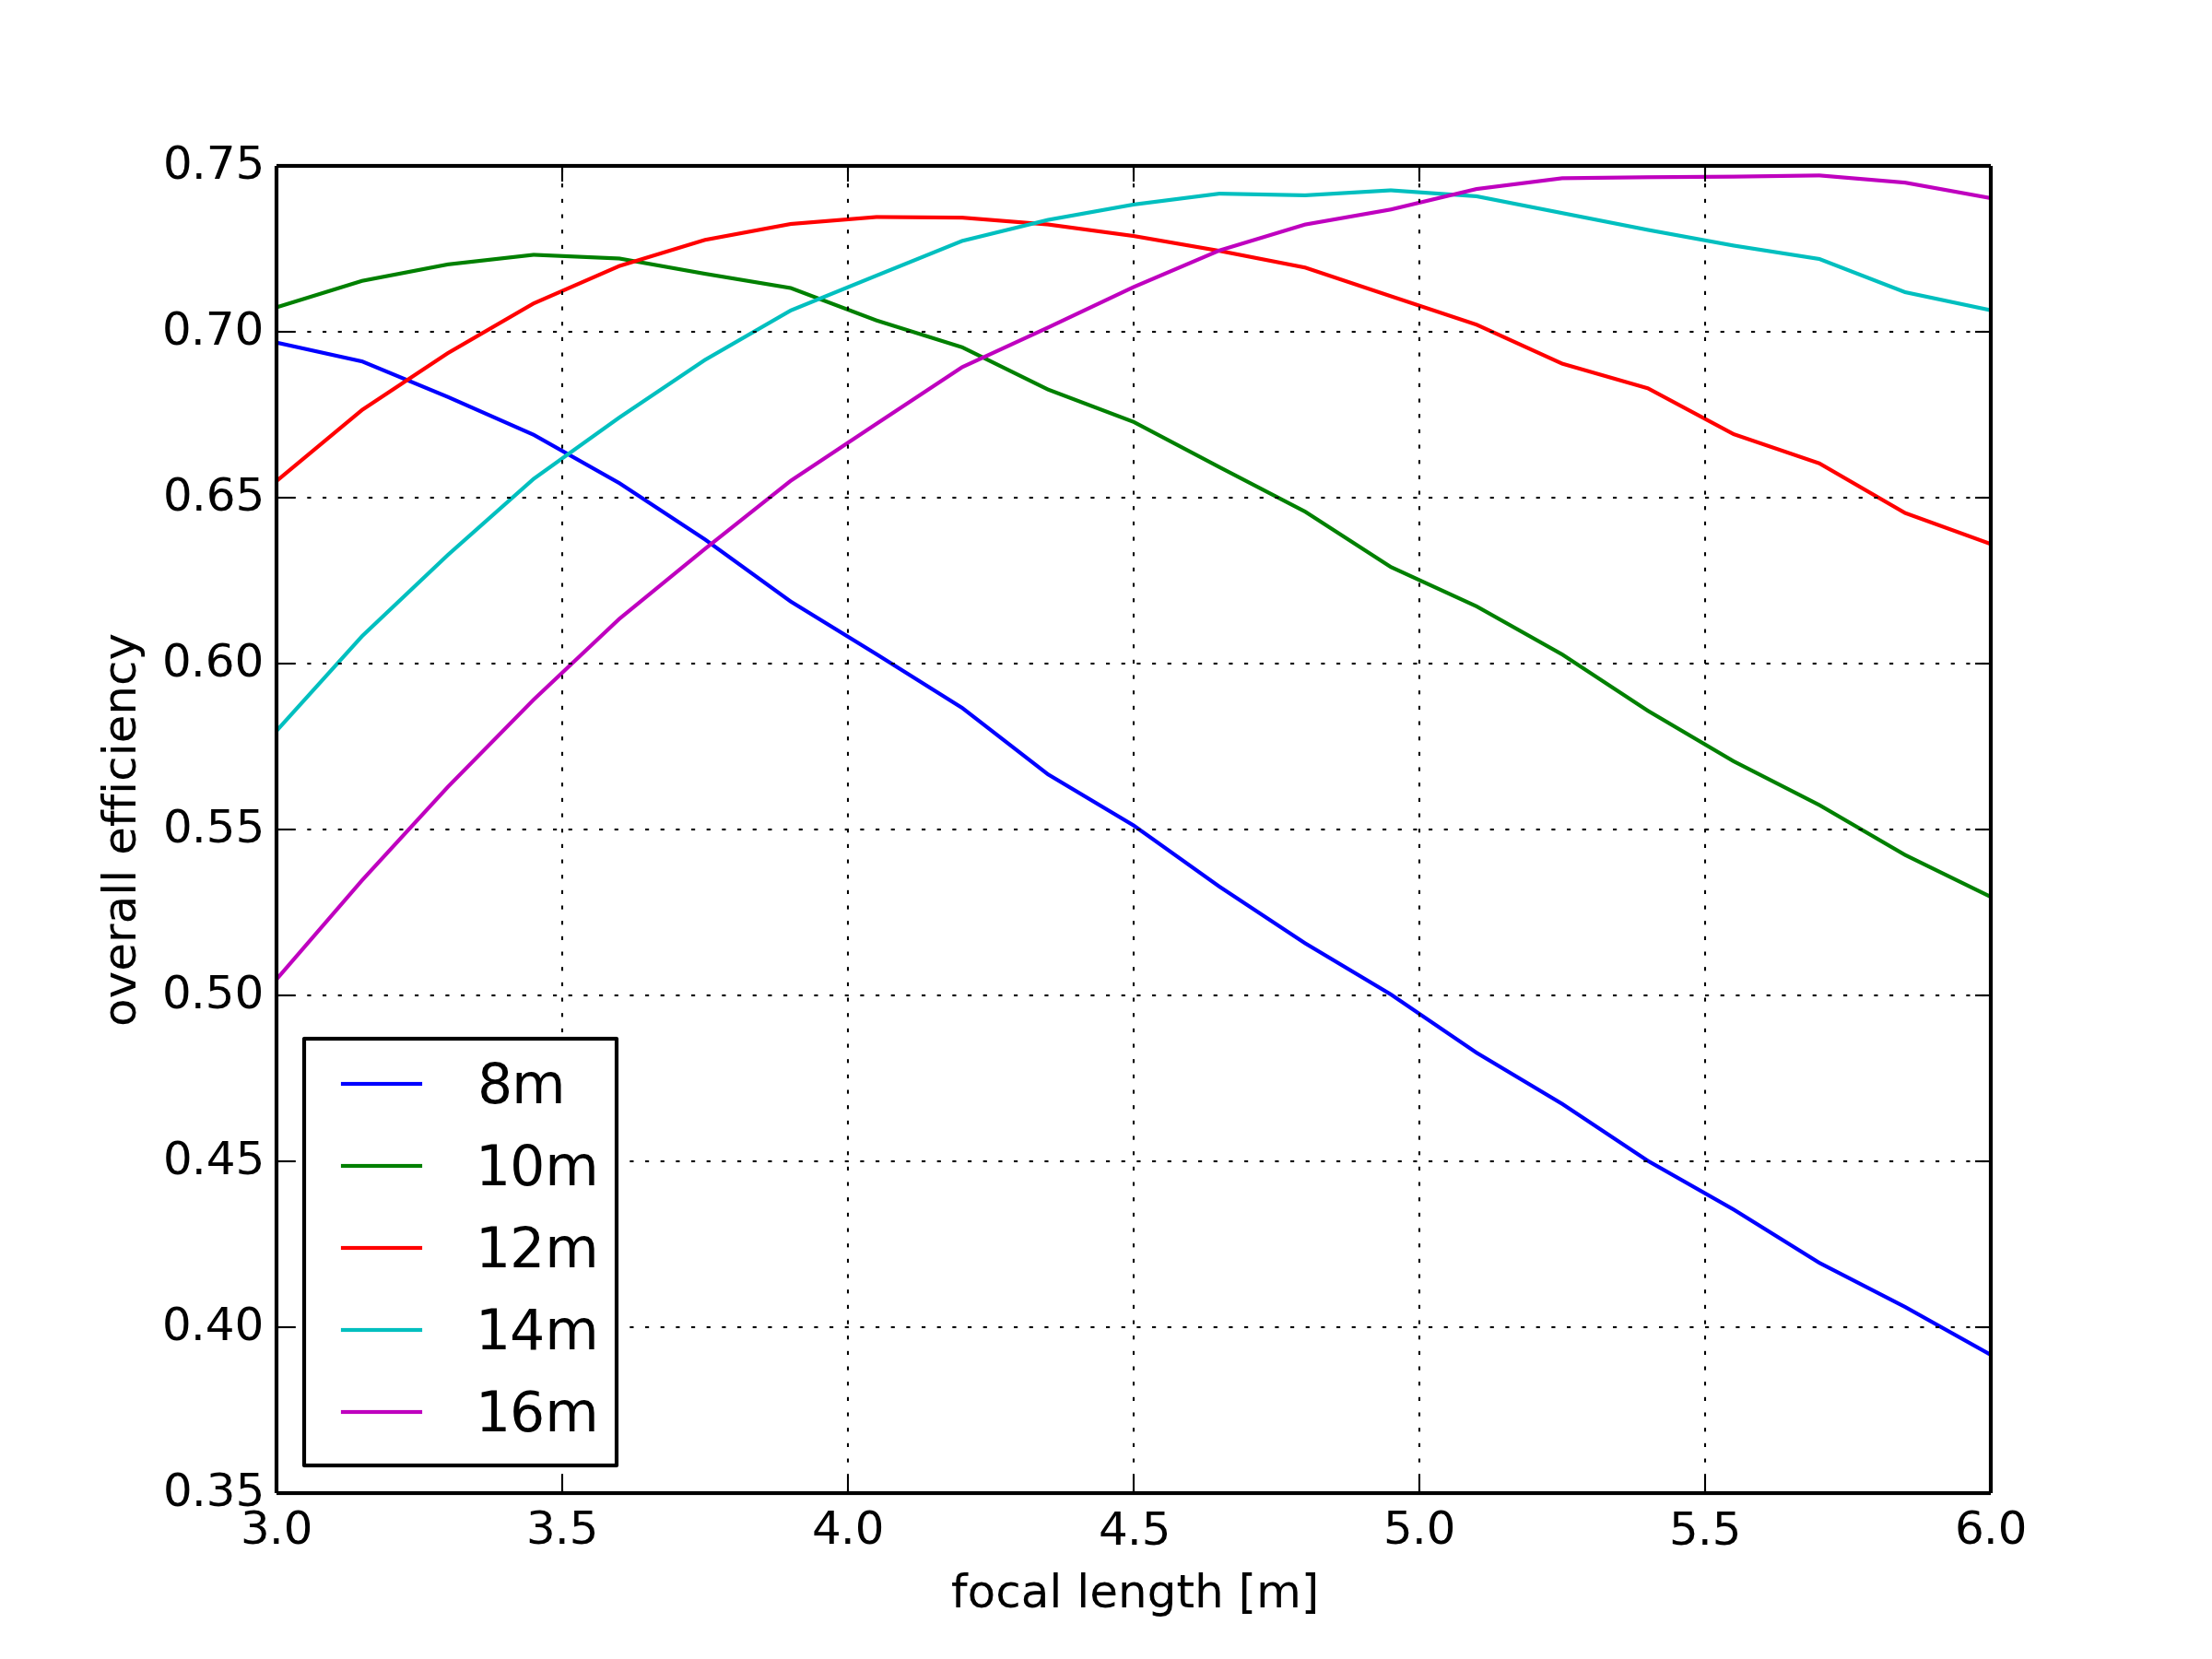
\includegraphics[width=0.8\textwidth]{plots/Engineering/focalEff.png}
		\caption{Analytical model efficiency of a parabolic element as a function of focal height and diameter.   The delay 
				contamination specification is $f<5$m.}
		\label{fig:disheffic}
	\end{subfigure}
	\caption{Cost and performance variational analysis data for the element.}
\end{figure}

% FOLLOWING SEEMS TOO DETAILED FOR A PROPOSAL
%To distinguish between measured sky delays and instrumental-induced delays at a required threshold ($R_T$) dB, 
%we need sufficient attenuation of the reflected signals at a given focal length ($f$) at a specified delay ($\tau_{d}$).  Assuming a conservative simple model that the magnitude of the reflection is attenuated by $A$ dB at each reflection 
%we see that for a delay length limit of $\delta_{d}=c\tau_{d}$ and focal length $f$,  the required focal length is
%
%\begin{equation}
%f < \left(\frac{A}{R_T}\right)\delta_d.
%\end{equation}
%
%Using nominal values of $R_T$ =  60dB (an order of
%magnitude below where EoR is predicted to be below foregrounds) at delays
%corresponding to the time it takes travel 15m and a net attenuation of 20 dB per reflection, 
%we find that the focal length should be less than about 5 m.  Free-space loss effects would 
%increase that value, loosening the constraint.
%DETAILEND

To maximize sensitivity, we wish to maximize the efficiency of the
HERA element, while still thresholding the delays at which reflections couple
back into the feeds. The design for the proposed HERA element is currently set
at $14m$-diameter dish with a focal height of $4.5$ m, which currently gives us
good total efficiency (see Fig \ref{fig:disheffic}) while staying within the delay-response constraint. 
Analytical models of the beam pattern are shown in Figure \ref{fig:beam}.
Full electromagnetic modeling will be coupled with 
physical measurements of the prototype to validate and refine the element.

%In addition to the constraints given by the element itself, the HERA element size is
%also influenced by the location of the ``knee'' in the EoR power spectrum \citep{lidz_et_al2008}
%The EoR power spectrum has an upward slope for low $k$-modes which levels off
%around $k=0.15 h$/Mpc %(see fig blah). 
%Working inside this $k$-mode would be beneficial due to the fact foregrounds are
%less problematic. This poses a problem because without knowing the
%width of our foregrounds, we can't say for sure which $k$-modes (in the power
%spectrum) are corrupted. This uncertainty, coupled with increasing systematic affects for shorter 
%baselines (hence smaller diameters), favors larger diameter antennas.

% AAARRGGHH!
\begin{figure}[h]
	\centering
	\begin{subfigure}[b]{0.46\textwidth}
		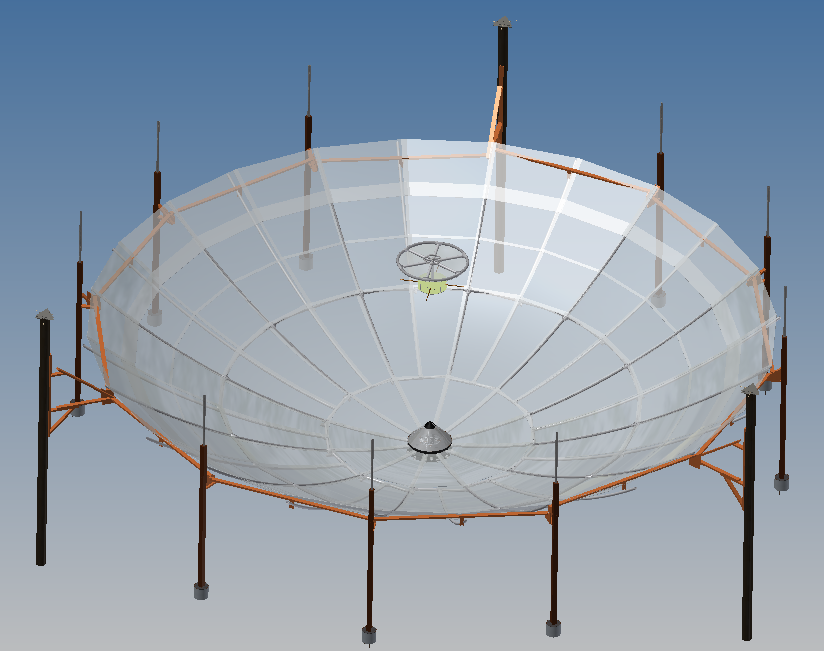
\includegraphics[width=0.85\textwidth]{plots/dish.png}
		\caption{CAD model of 14m dish with screening and some supports removed to show detail.}
		\label{fig:dish} 
	\end{subfigure}
\quad
	\begin{subfigure}[b]{0.46\textwidth}
		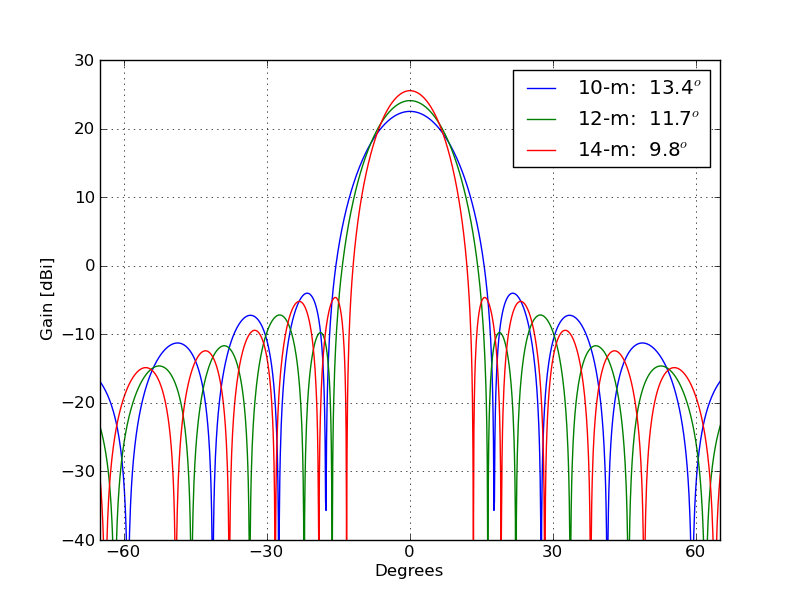
\includegraphics[width=\textwidth]{plots/Engineering/hera_beam.png}
		\caption{Analytical model beam patterns at 10m, 12m and 14m.}
		\label{fig:beam} 
	\end{subfigure}
	\caption{HERA element and beam pattern.}
\end{figure}

%The $k$-mode for a $14m$ baseline is $k = 0.023$, given by $k_{H} =
%\frac{B}{c}\frac{dk}{d\eta}$, where $B$ is the length of the baseline, 14m in
%our case, $c$ is the speed of light, and $\frac{dk}{d\eta}$ is the cosmological
%transfer function from delays to $k$-modes. In addition, narcissistic
%reflections add into our $k$ budget as well. The $f$ and $D$ choices above provide a $k$ budget for
%foreground widths to be within $\Delta{k}\sim{0.1}$. Testing these hypothesis
%and again, finding a compromise between maximum sensitivity, foreground budget
%will be key to testing and constructing the required element. Foreground width constraints
%are still an area of active research \citep{pober_et_al2013}.

The core defining elements in this design are the central hub and three tall support poles.  Three intermediate 
support posts are installed between each pair of poles.  A 2$^{\prime\prime}$ PVC spar of 24.1$^{\prime}$ 
terminates at each pole and post.  These spars are supported at each end and one point in the middle at the 
proper height and angle.  The intervening PVC pipe essentially acts as a smoothing filter between those 
points, noting also that a beam with point loads attains nearly the quadratic shape desired.  The CAD model is 
shown in Figure \ref{fig:dish}.  

The tall ($\sim$ 7m) poles provide locational accuracy (in all three dimensions) for the overall array installation.  
Using conventional commercial pole-installation techniques the poles are installed first for the entire array.  
Note that every pole except for the edge poles are shared by three antennas.  A standard theodolite can 
then be used to mark a known level height on all three poles.  These locations are then used with tensioned 
lines to define the center of that element and the hub is positioned at that location using a jig.

The hub uses concentric commercially available ``sonotube'' forms (circular cardboard forms for concrete pillars) 
and PVC sleeves to hold the PVC spars and PVC supports.  The retaining holes may be accurately cut into 
the forms, sleeves installed and concrete poured to make a simple hub to the desired accuracy.  The jig holds 
the concentric rings in place and allows it to be centered by tensioned lines while the concrete is poured.  
When the concrete cures one can then transfer an accurate offset from the dish vertex back to the poles.
The intermediate posts are then located by the support sub-assemblies attached to the poles and posts along 
with the rim sub-assemblies.  These are positioned and a small pier is poured to locate them.  After spar support 
pieces are installed on the posts, the spars themselves and the metal cloth can be installed.

The feed is held off the three tall poles using tensioned lines to accurately locate it over the hub.  A precise 
length of kevlar rope holds the feed down to the hub at a precise focal point.  The RF cables follow the line 
down and out to the analog-to-digital converters and correlator.  

To minimize cross-talk, metal screens are strung between every pole/post, which go to the level of the feed.  
The dishes have a rim-to-rim spacing of 30cm to allow the screen to be slightly angled to minimize standing waves.

% XXX
====> There is nothing on the configuration yet.

\vspace{-0.25in}
\subsubsection{Signal Path}
\vspace{-6pt}
The signal path will utilize the front-end and post-amplifier gain modules directly
from PAPER, although additional studies will be carried out to improve the feed
response below 100 MHz. The amplifier/baluns and post-amplifier modules already have
the ability to work over an extended lower end. The front-end amplifier has a low
noise figure with moderate gain, high dynamic range to tolerate RFI, unconditional
stability to ensure oscillation-free operation, well-matched impedance to both the
antenna and cable, well-understood temperature dependence, a mechanically rugged
mechanical design, low susceptibility to electrostatic discharge, low power
consumption, and low fabrication cost. It is housed in a metal enclosure affixed to
the antenna to form a very rugged, reliable, low-cost unit with excellent RF
performance \citep{parsons_et_al2010}.

% AAARRGGHH!
\begin{figure}[h]
	\centering
	\begin{subfigure}[b]{0.3\textwidth}
		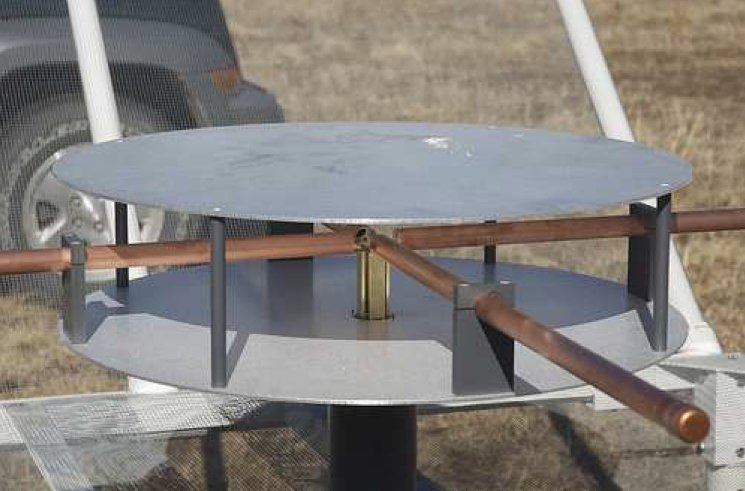
\includegraphics[width=\textwidth]{plots/new_antenna_closeup.jpg}
		\caption{Photograph of the PAPER antenna positioned above the trough reflector.}
		\label{fig:element}
	\end{subfigure}
	\quad
	\begin{subfigure}[b]{0.3\textwidth}
		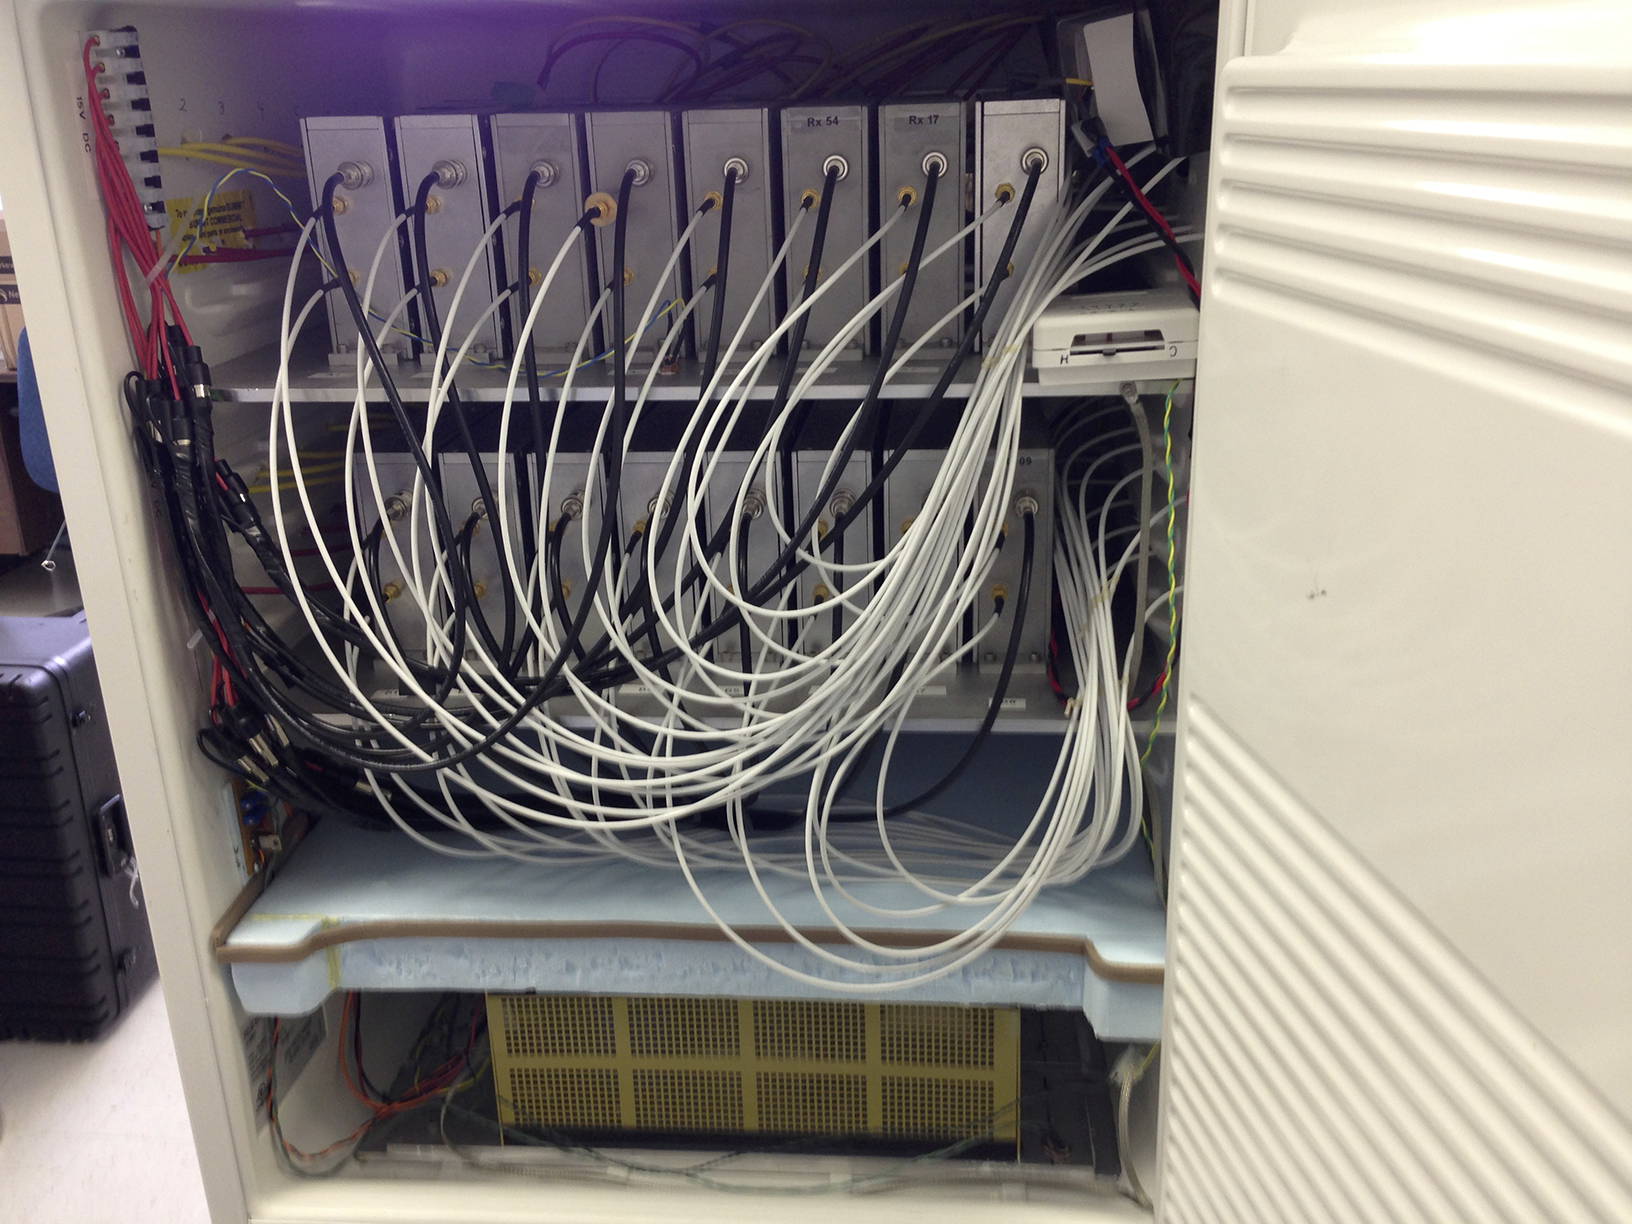
\includegraphics[width=\textwidth]{plots/Engineering/recv_node.png}
		\caption{Receiver modules in a node refrigerator.}
		\label{fig:recv_node} 
	\end{subfigure}
	\quad
	\begin{subfigure}[b]{0.3\textwidth}
		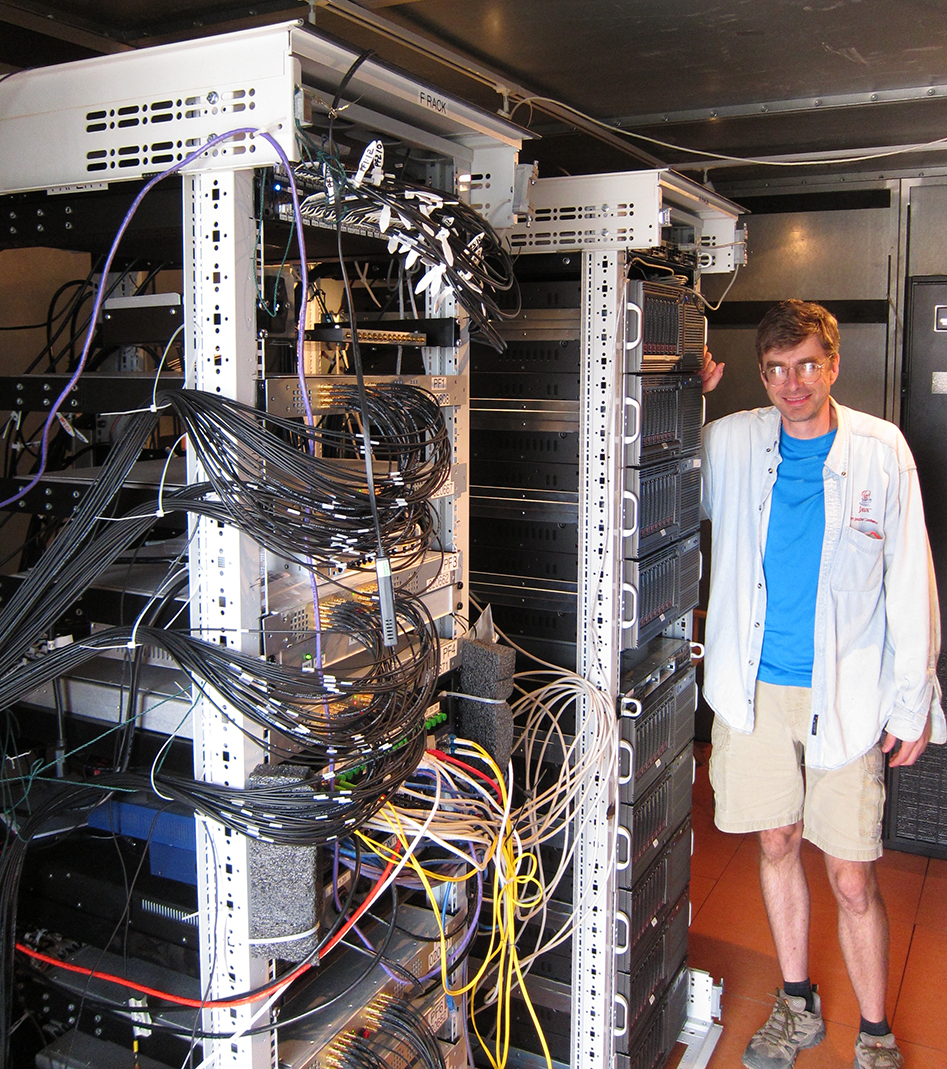
\includegraphics[width=0.8\textwidth]{plots/Engineering/digital.png}
		\caption{Digital equipment (ADC/correlator) in container.}
		\label{fig:digital} 
	\end{subfigure}
	\caption{Photographs of existing instrument components to be used.}
\end{figure}

The signal is transported to the node via a 35-meter run of 50 $\Omega$ coaxial
cables. It will terminate on a bulkhead plate on the face of the RFI-tight and
air-conditioned node. Inside, dual-channel post-amplifier modules (PAMs) (Fig.
\ref{fig:recv_node}) amplify and band-limit the signal. Inside the RFI-tight node,
the PAMs themselves are housed in RF-shielded boxes.

A new board called the Smart Network ADC Processor (SNAP) board, to be incorporated 
into the CASPER suite of hardware and firmware, is currently in layout at NRAO.  SNAP
takes the output from the PAMs, digitizes and channelizes it before putting it on optical fiber
for transmission to the Karoo Array Processing Building.

\vspace{-0.25in}
\subsection{Prototype Construction and Testing}
\vspace{-6pt}

One prototype of the antenna has been constructed near the Radio Astronomy Lab in California. 
This prototype serves as an important first construction test-bed and is currently being used to do 
initial network analyzer measurements (Fig. \ref{fig:heracles}).
This proposal calls for the construction of two additional prototype dishes alongside
the PAPER array deployed at the NRAO site near Green Bank, WV.
These dishes will be tested
with a network analyzer in situ, and will be cross-correlated with PAPER elements using
the correlator currently deployed on site, in order to measure
the element performance and optimize the design.  The goal of this effort is to ensure
that all signal reflections
are attenuated by a factor of -60 dB by the time that they are capable of entering the signal path
at a delays greater than 50 ns.  While signal reflections will be inevitable with such a dish
design, the quality of the impedance match at the feed,
the presence of structures that reduces resonances between
the feed and the dish, and control of the focal height of the parabola are all aspects
of the design that can
be manipulated to help achieve this specification, ensuring that reionization modes above
$k_\parallel=0.1h {\rm Mpc}^{-1}$ are not dominated by foreground contamination.

% AAARRGGHH!
\begin{figure}[h]
	\centering
	\begin{subfigure}[b]{0.46\textwidth}
		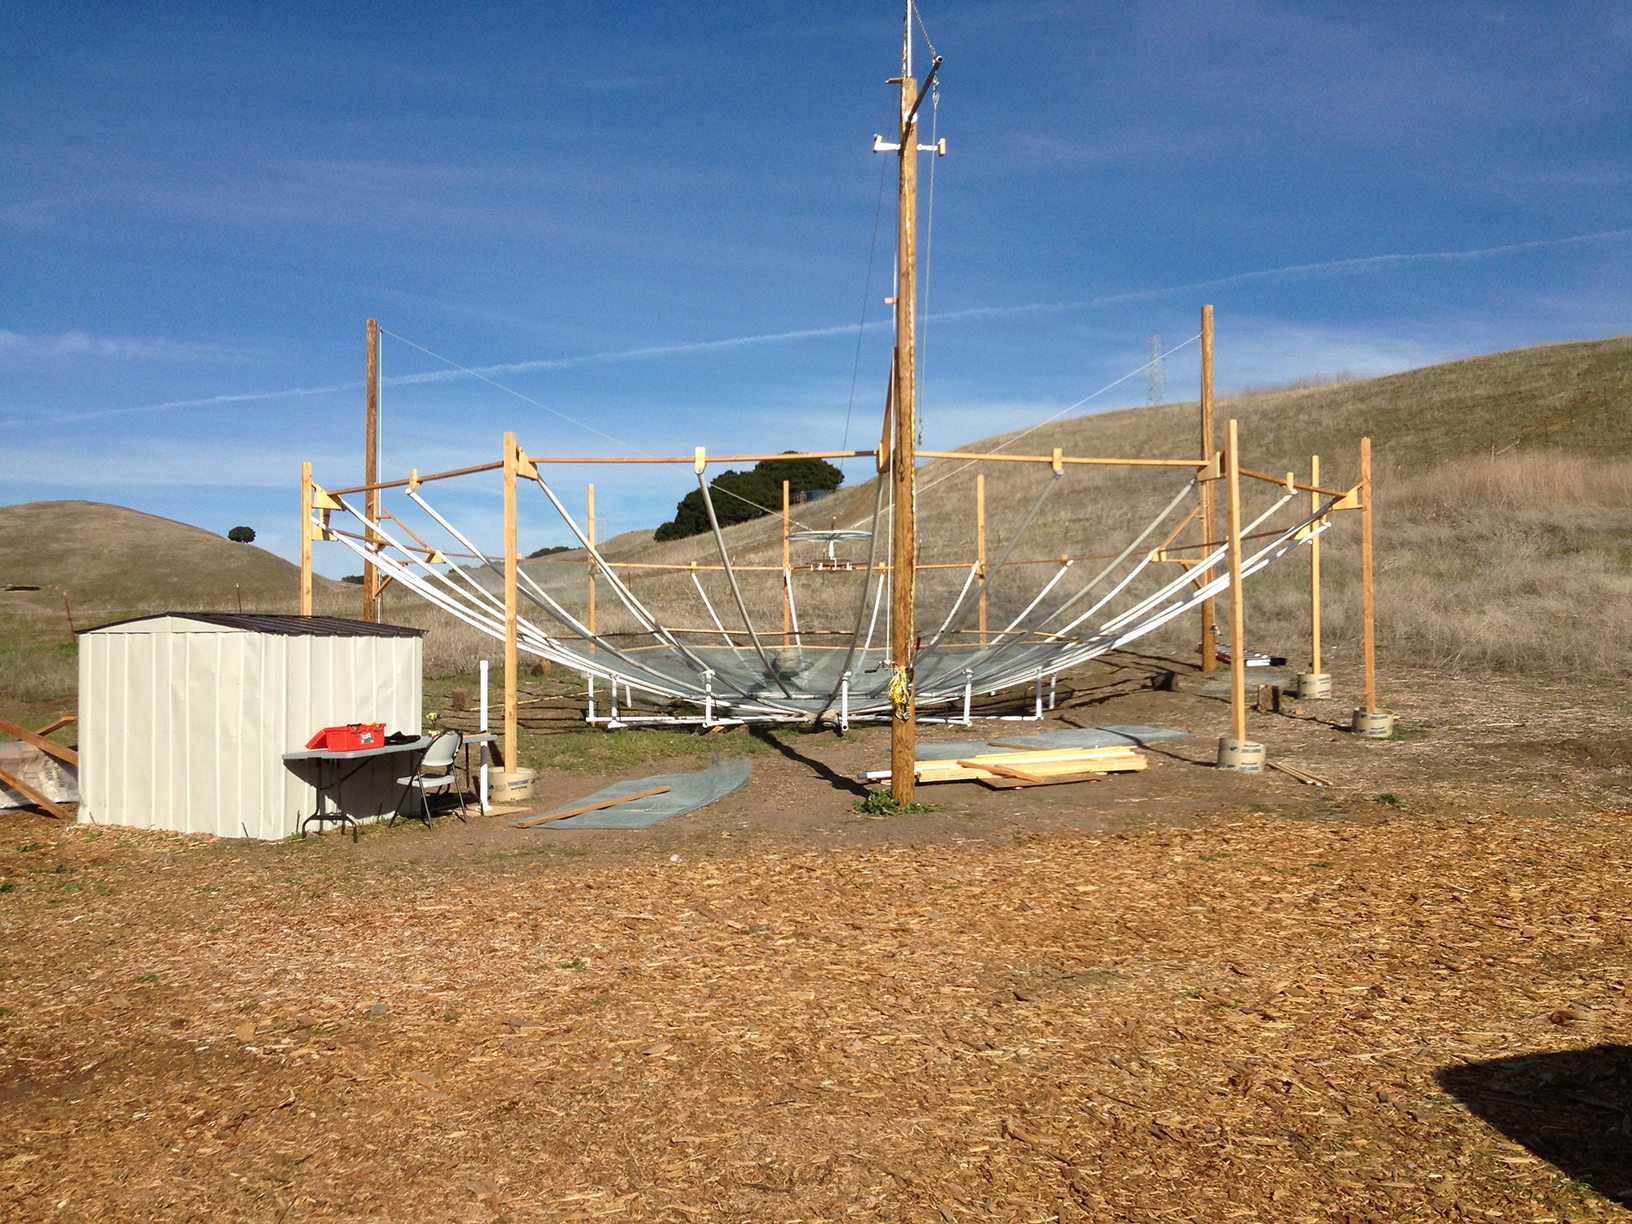
\includegraphics[width=\textwidth]{plots/heracles.png}
		\caption{Picture of the existing construction prototype in California.}
	\end{subfigure}
	\quad
	\begin{subfigure}[b]{0.46\textwidth}
		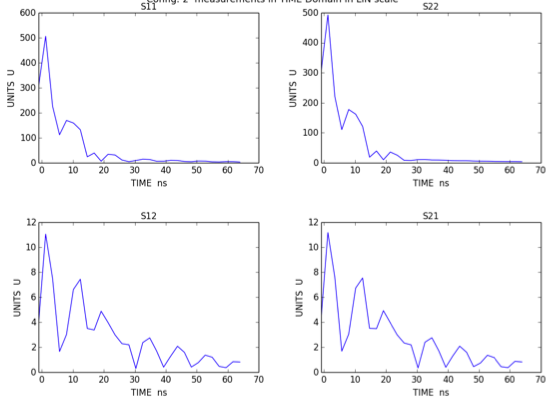
\includegraphics[width=\textwidth]{plots/Engineering/heraclesNA.png}
		\caption{Initial reflection measurements from the prototype.}
	\end{subfigure}
	\caption{Prototype antenna and initial results.}
	\label{fig:heracles}
\end{figure}

These additional prototypes will be important to finalize the specific construction techniques to be 
used in the final antenna construction contract in South Africa.

\vspace{-0.25in}
\subsection{Array Construction}
\vspace{-6pt}
Construction of HERA-61 consists of five primary steps: 
\begin{enumerate}[noitemsep,nolistsep]
\item site preparation and surveying 
\item pole installation by contracted labor with specialized utility pole equipment 
\item hub placement and height adjustment
\item remainder of construction of each element, following description above, using local labor 
\item moving the feeds and cables from the existing PAPER dipoles to new ground screens by project staff
\end{enumerate}

The contractors and immediate supervisors will be based in South Africa.  Supervision staff 
will be part of the extensive support infrastructure in place at the site to support South African SKA activities.
As mentioned above, the tall poles are shared amongst the antennas in the tight configuration.  
Therefore, 61 antennas requires only 75 poles rather than 61x3=183.  These are standard telephone/power 
utility poles and a great deal of  expertise and infrastructure exists to install these in remote settings.  
Figure \ref{fig:config} shows the configuration of the 61 antennas including the tall pole locations and \ref{fig:optics} shows a cross-section of an element.

% AAARRGGHH!
\begin{figure}[h]
	\centering
	\begin{subfigure}[b]{0.35\textwidth}
		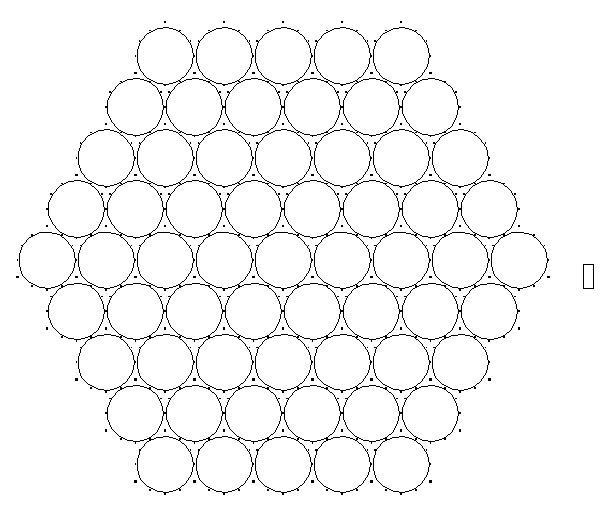
\includegraphics[width=\textwidth]{plots/Engineering/hex_61.png}
		\caption{Configuration of the 61-element array.  Note the rectangular container to scale on right.}
		\label{fig:config}
	\end{subfigure}
	\quad
	\begin{subfigure}[b]{0.6\textwidth}
		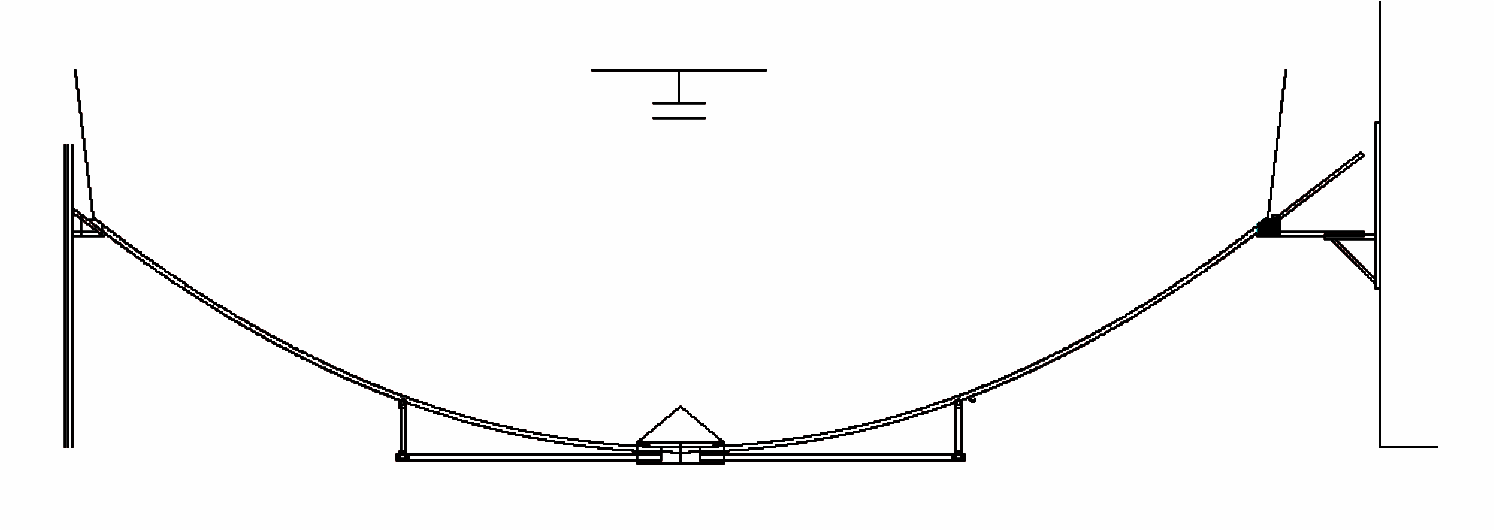
\includegraphics[width=\textwidth]{plots/Engineering/optics.png}
		\caption{Cross-section and optics of an element.}
		\label{fig:optics}
	\end{subfigure}
	\caption{Configuration and optics.}
	\label{fig:config_optics}
\end{figure}

Except for two custom metal assemblies, the remainder of the construction materials are standard wood, 
metal and PVC parts.  The two custom assemblies are simple small welded metal assemblies for the end of 
rim support pieces (quantity 12) and the feed and feed backplane (quantity 1).  The PVC and wood sub-assemblies 
will be constructed off-site where material and labor is readily accessible and shipped to site.  The 
construction of these sub-assemblies, pre-cut wood and PVC, and wire mesh pieces will be done on-site under 
contract.  Project staff will then move over the existing PAPER feeds and cables and commission the array.  

\vspace{-0.25in}
\subsection{Commissioning}
\vspace{-6pt}
Note that since all of the electronics are already deployed and working, commissioning will consist of verifying the existing performance but within the new electromagnetic environment presented by the new ground screens.  Below is
an explicit list of commissioning tasks:
\begin{itemize}[noitemsep,nolistsep]
\item equalization of signal levels and repairing of reflections and misbehaving signal paths due to cabling using auto-correlation data 
\item measure system temperature from raw level of auto-correlation data as it varies diurnally.
\item measure relative width of primary beam using source transits for XX and YY polarizations 
\item use established sky model from PAPER and correlation with known PAPER feeds to 
determine absolute gain as a function of direction for new dishes. 
\item use redundancy to solve for phase and gain calibration parameters, measure stability of parameters versus 
time 
\item detailed characterization of cross-coupling and reflections between antennas using cross-correlation data and imaging 
\item fold calibrated data on the basis of redundancy and multiple observing days to obtain a high-sensitivity delay spectrum capable of verifying absence of low-level reflections at higher delays. 
\end{itemize}

%%%%%%%%%%%%MRI VERSION
%%%%%%%%%%%%%%%%%%%%%%%%%%%%%%%%%%%%%%%%%%%%%%%%%%




\subsubsection{Analog System}
ii. 14m elements + broad band (active) dipole feed
% de Boer, Bradley

\subsubsection{Digital System}

Digital signal processing (DSP) electronics --- particularly the digital correlator ---
have historically been one of the most complex and expensive aspects of any radio interferometer.
Correlators have commonly been
developed independently for each project, with a substantial investment
of time and money to engineer
custom solutions for hardware, physical interconnect,
communication protocols, and control software. The complexity of such development
leads to lengthy incubation times and an
associated loss of timely scientific research. Furthermore, the large
engineering investments involved leave few resources
for upgrading systems that fall quickly into obsolescence as a result
of Moore's Law.

\begin{figure}[!ht]\centering
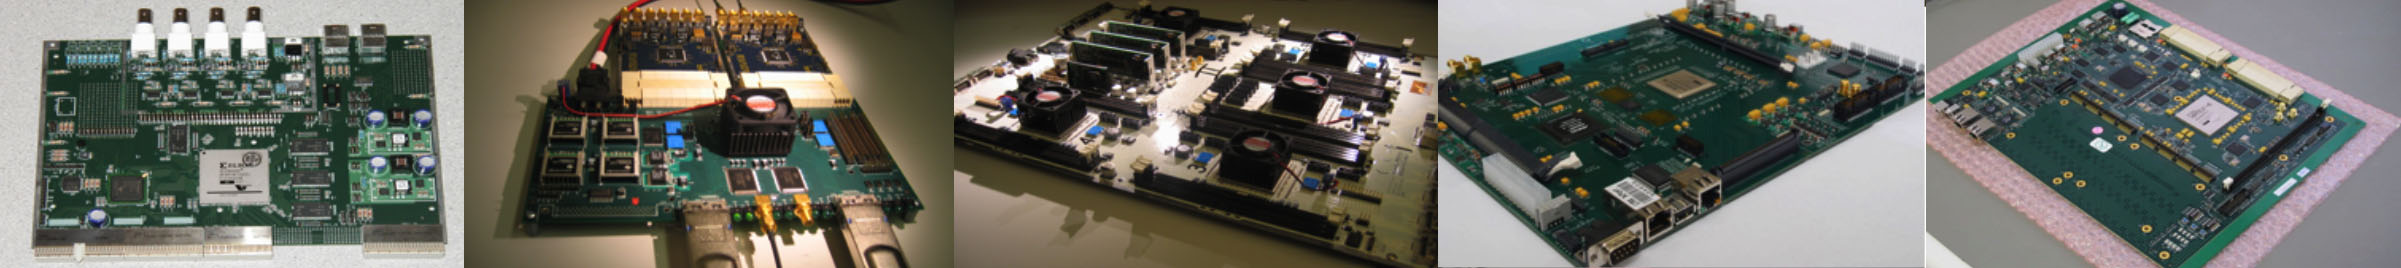
\includegraphics[width=6.5in]{plots/casper_boards.jpg}
\caption{
Five generations of CASPER technology (progressing left to right) have been used to rapidly
develop, test, and deploy DSP instrumentation for radio astronomy.  Correlators,
beam formers, and spectrometers all use a common set of hardware modules, along with a library
of parametrized DSP algorithms, that can be easily upgraded to incorporate new technology
\citep{parsons_et_al2006,parsons_et_al2008}.
}\label{fig:casper_boards}
\end{figure}

This is changing.  The Collaboration for Astronomy Signal Processing and Electronics Research
(CASPER; \citealt{parsons_et_al2006}) was founded seven years ago at Berkeley
by Werthimer and Parsons as a program 
to open-source and share the development of real-time signal processing engines for astronomy.
CASPER now has world-wide participation that is
transcending the radio astronomy community to include physics, engineering,
medical, and genomics research, with
over 500 members at 73 institutions, and, as illustrated in
Figure \ref{fig:casper_boards}, five generations of DSP hardware.
% XXX something about GPUs here?
As a result of the CASPER's cumulative body of open-source hardware designs, DSP libraries, instrument
architectures, and control software,
correlator development --- formerly the Achilles heel of building interferometers ---
is now widely viewed as a solved problem.  PAPER, on a modest budget, has developed and deployed new correlators
annually for five years running, each quadrupling the computational capacity of its predecessor.
HERA will continue this incremental development cycle, following the packet-switched
FX correlator architecture described in \citet{parsons_et_al2008} that has been
extended in recent PAPER and LEDA deployments to rely on a heterogeneous system FPGA and graphics processing units (GPUs)
to efficiently achieve the required data processing bandwidth \citep{clark_et_al2012}.

Under HERA, this correlator architecture will continue to evolve.  In order to meet HERA's science requirements,
which specify that the analog signal path must be shorter that XXX m in order to limit the time constant of any signal reflections
that arise in the system, digitization at the front-end of the correlator must occur in the field, close to the antenna
elements.  This specification, along with a growing need for modularity to scale with the number of parallel signal paths,
lead HERA to adopt a node-based architecture for amplification, digitization, channelization, and digital
transmission in the field that builds on HERA's MWA heritage.  This architecture is merged with PAPER's clean 
architecture for real-sampling and channelizing the entire analog passband at once, packetizing the data into
10 Gb Ethernet format, and relying on commercial switches to perform the frequency/antenna corner-turn that is
FX correlator architectures require. 

\paragraph{Node}

\begin{figure}[!ht]\centering
%\includegraphics[width=6.5in]{plots/node_arch.png}
\caption{
XXX something about nodes here.  Maybe also block diagram of NRAO digitizer board.
}\label{fig:node_arch}
\end{figure}

HERA's nodes each consist of a single, RFI-tight enclosure housing 16 dual-polarization receiver modules, 
6 data acquisition (DAQ, XXX or whatever we call them)
modules, power supplies, cooling, and small server for monitor and control (see Figure \ref{fig:node_arch}).  HERA-331 will employ
21 nodes (XXX probably more like 25), each capable of processing the signals from 16 antenna elements.
DAQ modules, which are currently under development, and are in the advanced stages of schematic design and layout,
act as both the digitizer and F-Engine in HERA's FX correlator architecture.  Each DAQ
is responsible for digitizing 6 input signals (3 antennas, dual-polarization) at a rate
of 500 Msps, for a Nyquist bandwidth of 0--250 MHz.  This band is channelized into 2048 channels
using a Polyphase Filter Bank running on the DAQ's relatively inexpensive Xilinx Kintex XXX FPGA.
The FPGA forms data packets out of 100 MHz of channels selected throughout the band, each represented
with an 8-bit fixed-point complex number.  The aggregated bandwidth of 4.8 Gbps per board is transmitted in
10-Gb Ethernet format over a single SFP+ port, through a XXX optical transceiver module, onto an optical
fiber that runs back to a central container adjacent to the array.  
% XXX don't know if this next part is strictly necessar to say, or just cute.
This transmitted bandwidth is approximately
half of the link capacity; the spare capacity will support a transmitted bandwith
of 200 MHz in the event that Moore's Law delivers X-Engine processors capable of support
this additional processing when they purchased in the third year of the project.

\paragraph{Central Container}

HERA's central container houses two significant subsystems.  The first is a timing subsystem
that is responsible for maintaining a GPS-disciplined oscillator and distributing timing
signals (the sampling clock and 1PPS synchronization) to each of the nodes.  The second
subsystem is a straight-forward passive fiber optic patch panel that is responsible for coupling
the optical network attached to the nodes into a 192 (XXX)-filament optical fiber bundle
% XXX need to check costing again on full parallel tx vs color mux with tuned transceivers
that attaches the container to the downstream portion of the correlator system.

\paragraph{Karoo Array Processing Building (KAPB)}

The KAPB is currently
in advanced stages of construction for MeerKAT, and will house the switch and X Engines that
complete the HERA correlator system.  The fiber optic bundle that enters the KAPB will patch
into local fiber optic cables 
% XXX and possible demux here
that each terminate in optical transceivers that plug into a 240-port (XXX) 10 GbE switch.
Such switches, while large, are readily available commercially today.  Also connected to
this switch are 30 servers, each hosting two dual-GPU graphics cards and two dual
10 GbE network interface cards, which implement the cross-multiplication (X-Engine) component
of the correlator during observations.  This estimate for the number of X-Engine servers
is extrapolated from current GPU servers deployed on PAPER, assuming no improvement in bus
speeds for transfering data into the GPU cores, but assuming that the computational
capacity of such GPU cores doubles according to Moore's Law prior to the purchase of
these servers in the third year of the project.

Assuming 8-second integrations from the correlator, the raw data output of the
correlator while operating will be, assuming a 100-MHz correlated bandwidth, 1.8 Gbps.
These raw visibilities will be assembled in order by four servers
and recorded to a XXX TB RAID storage system at full rate in the Miriad UV
file format.

\subsubsection{Data Storage, Compression, and Transfer}

HERA's storage system in the KAPB will have the capacity to store all raw observations
(XXX TB) for a 180-day observing season.  However, PAPER has implemented a data compression
scheme (see Appendix A of \citealt{parsons_et_al2013}) that can be applied to HERA visibilities
to reduce data volume by approximately a factor of 20 without impacting reionization science capabilities.
This compression technique, which is based on delay/delay-rate filtering \citep{parsons_backer2009},
is applied uniformly to all visibilities in the array, and does not require (or produce) detailed 
calibration information.  As a result, this compression scheme is robust against gaps in
real-time knowledge of the array, and minimally restrictive in how the data
are analyzed and calibrated afterward.  As with PAPER, we plan to apply this compression
automatically to HERA observations to reduce data volume, and lower the computational demand
of subsequent analysis.

Data compression, while not as computationally demanding as other data reduction schemes
that have been proposed, does nonetheless incur a substantial computational burden.
HERA does not plan to conduct daytime observations, owing to the level of interference
introduced by the active Sun.  As a result, HERA's X-Engine servers will only operate
at night, leaving them available to work on data compression during the
daytime.  Leveraging the capacity and flexibility of their graphics cards for high-performance
computing, these servers will read back the previous night's observations, perform RFI flagging,
apply the necessary transformation and filtering, and will output compressed visibility data
back to disk.

% XXX need to discuss the plan for how data are shipped over to UPenn here. see below

C. Post correlator data path
% Aguirre, Moore

i. local storage

ii. transport to data centers

iii. data centers: access? 

\subsection{Analysis}
D. Data analysis [Move up?]

i. Calibration 
% Aguirre, Morales

ii. Continuum and removal
% Morales

iii. Delay spectrum analysis
% Pober

iv. Other (related) approaches: Bayes, z-variance,
% Liu, Carilli

v. HI imaging
% Jacobs

E. Array monitoring/maintenance: daily, weekly health monitoring
% de Boer

F. Aspirations [move to facilities section?]

i. FFT correlator

ii. other

\subsection{Five year Schedule and deliverables} % 0.5 page
% De Boer

i. stages and science

ii. first science within 3 or 4 years

iii. main science results before end of decade


\section{Broader impacts} % 1 page
% Aguirre

A. pre and post-doctoral students

%B. South Africa connection
\subsection{South African Connection}
%i. professional development/exchanges

\subsubsection{Student Exchange}

We propose to broaden the scientific and technical impact of HERA by a program of student exchange between HERA and South African scientific collaborators.  This exchange is intended to be a mutually beneficial experience, with students on both sides being prepared to be world leaders in astronomy, and particularly in future work with next-generation 21 cm reionization experiments, and with the Square Kilometre Array (SKA).

Experience has shown that students benefit tremendously from peer mentoring and a sense of community, particularly when operating in a new cultural environment.  This is similar to the approach taken for South African students in their National Astrophysics and Space Science Programme (NASSP)
%; http://www.star.ac.za/) 
and also in US programs (e.g., the Posse Foundation).
%http://www.possefoundation.org/).  
Our student exchange program would pay special attention to bridging issues of scientific culture, allowing both groups to function at the highest possible level within their exchange community.  We anticipate that this program will prepare students on both sides to be able to productively apply for graduate, postdoctoral, and faculty positions in the exchange country, and to effectively apply for observing time on the SKA and NRAO facilities.  The net effect is an increase in the size and diversity of the talent pool.

The SKA SA has been consciously and actively prioritizing support to previously disadvantaged South Africans.  A deliberate focus is on addressing gender and race inequality in science and engineering at all levels, by prioritising support to black and women South Africans at undergraduate level, and guiding and supporting them into higher levels of research.  The undergraduate programme is designed to identify and support black and women South Africans at undergraduate level, and motivate them to continue into postgraduate research. The level of financial support provided by the project at all levels of study and research ensure that the students do not have to concern themselves with finding employment immediately after graduating from a degree, a problem faced by many students who have obligations to contribute to their families’ income.

Specifically, we propose that each year of the grant, an exchange would be organized around a group of students (3 – 4) from each of the USA and RSA who would travel to a specific exchange institution to work on a related set of research problems over the course of a 3 month period (e.g., the northern summer).  These students would interact with both the host institution’s faculty and also the postdoctoral and graduate researchers there. For students in a Master’s program, this might represent their only exchange, and they would be mentored on application into PhD programs or engineering positions.  PhD candidates would participate in multiple exchanges, with the goal of establishing a sufficient scientific presence in their host country to apply to build post-graduate collaborations, apply for postdoctoral or permanent positions, and be in an excellent position to make good use of the host country’s radio astronomy facilities.  In order to vary the experience, each year would have a different host institution on each side, subject to the availability of mentors.

%ii. broader outreach in SA
\subsubsection{Broader Outreach in SA}

PAPER has an admirable history of enlisting interns from South African
universities as part of major engineering deployments, with the work
applied as practical training within their academic program.

C. Broader astronomy community

i. Data access: transients, SETI, ionosphere

ii. Cross correlation: CMBpol, CO/CII IM

D. Casper open source: good example to build from


\section{VI. Summary: why us and why now?} % 0.5 pages
% Parsons

This HERA proposal follows the vision for 21-cm observations laid out in NWNH.
PAPER and the MWA have already succeeded in the primary task envisioned in
NWNH---characterizing the astrophysical foregrounds and developing the hardware
and analysis 
tools needed to suppress the contamination. The discovery and
characterization of the EoR Window and the development of precision foreground
mitigation techniques have shown that foregrounds can be suppressed to the current
thermal noise level (\S \ref{LessonsSec}; \citealt{parsons_et_al2013}). While the MWA
and PAPER are pushing hard to detect the EoR power spectrum, %budget constraints have
%dictated that 
a marginal detection is the best these instruments can achieve.
HERA will both ensure a high significance detection of the \HI 21-cm 
signal as
well as provide powerful constraints on the rise and fall of reionization, how
early stars and structure formed, and physical processes at the end of the
cosmic dark ages (Figures \ref{fig:x_i_Xray} \& \ref{fig:eor_pspec}).

As envisioned in NWNH, the US EoR projects (PAPER, MWA, EDGES, MITEoR) have
pooled their expertise to develop the second generation HERA observatory. This
has created a collaborative team with a deep well of scientific
experience---the majority of papers on EoR observations are authored by members
of the HERA team. By leveraging this expertise, the HERA design is significantly
less expensive than envisioned in 
NWNH and has greater scientific reach.

The last few years have been remarkably productive---we
understand foreground systematics and are pushing 
existing
instruments to their thermal limits. We are now ready to build the HERA
instrument envisioned in NWNH and realize the scientific promise of 21-cm
cosmology.
Studying the formation of the first luminous structures 
and how they reionize the Universe is a primary driver for 
nearly all major astronomical facilities over the next decade.
Such studies include direct 
observations of stars, gas, dust, and AGN in the
first galaxies using the JWST, TMT, ALMA, and the JVLA. HERA is 
a unique and necessary element in this panchromatic arsenal, providing
providing the \emph{only} direct window onto the impact of these sources on 
their large-scale environments.


\clearpage
\setcounter{page}{1}
\thispagestyle{empty}
%\bibliographystyle{apj}
%\bibliographystyle{hapj}
\bibliographystyle{jponew}
\bibliography{biblio}

\end{document}

